\documentclass[a4paper,12pt]{scrartcl}

\usepackage[utf8]{inputenc}
\usepackage[ngerman]{babel}
\usepackage[T1]{fontenc}
\usepackage{graphicx}

\title{Webfleet TomTom}
\author{Christoph Behr, Greta Hellmann, et al.}
\date{01.April 2022}

\begin{document}
    \maketitle
    \tableofcontents
    
    \newpage
    \section{Einleitung}
    Das Programm Webfleet welches auf allen TomTom Navi's in unseren KTW's läuft gibt uns die Möglichkeit Einsätze sowie 
    alle dafür notwendigen Informationen einfach an die jeweiligen Besatzungen zu verschicken.
    Konsequent genutzt vereinfacht das Nutzen von Webfleet das Disponieren ungemein. Auch für die Besatzungen ergeben sich
    einige Vorteile. Dazu gehört eine bessere erreichbarkeit der Leitstelle z.B. für den Fall von Problemen im Einsatz die 
    nicht alleine vor Ort entschieden werden können oder auch zur freieren Arbeitsgestaltung. Dies soll eine "lebendige" Anleitung, die wir 
    zusammen erweitern und verbessern können, werden. So können wir hoffentlich unseren Arbeitsaltag möglichst entspannd verbringen.
    Leider sind mir noch nicht alle Funktionen von Webfleet bekannt, vieles von dem was das Programm kann ist sicher
    für uns auch nicht relevant. Sobalt mir oder euch Funktionen auffallen die genutzt werden können/sollen, wird diese Anleitung
    entsprechend geändert und erweitert. 
    Hier nun ein kleiner Überblick über das Annehmen und Bearbeiten von Einsätzen, sowie die manuelle Status gabe.
    
    \section{Bearbeitung von Einsätzen}
    Das standartmäßige vorgehen bei von der Leitstelle gesendeten Einsätzen ist einfach gestaltet. Sobalt der Einsatz von
    der Besatzung angenommen wird geht eine Meldung an die Leitstelle. Der Einsatz wird in CareMan (der von der Leitstelle 
    genutzten Dispositionssoftware) gestartet. Durch "weiter drücken" in Webfleet wird der aktuelle Status des KTW an die Leitstelle
    übermittelt. Wir gehen nun die einzelnen Schritte im Detail durch.

    \subsection{Annahme von Aufträgen}
    Die von der Leitstelle gesendeten Einsätze sind chronologisch geordnet im Hauptmenü zu finden.
    Wählt den aktuellen Einsatz aus.
    \begin{figure}[h]
        \begin{center}
            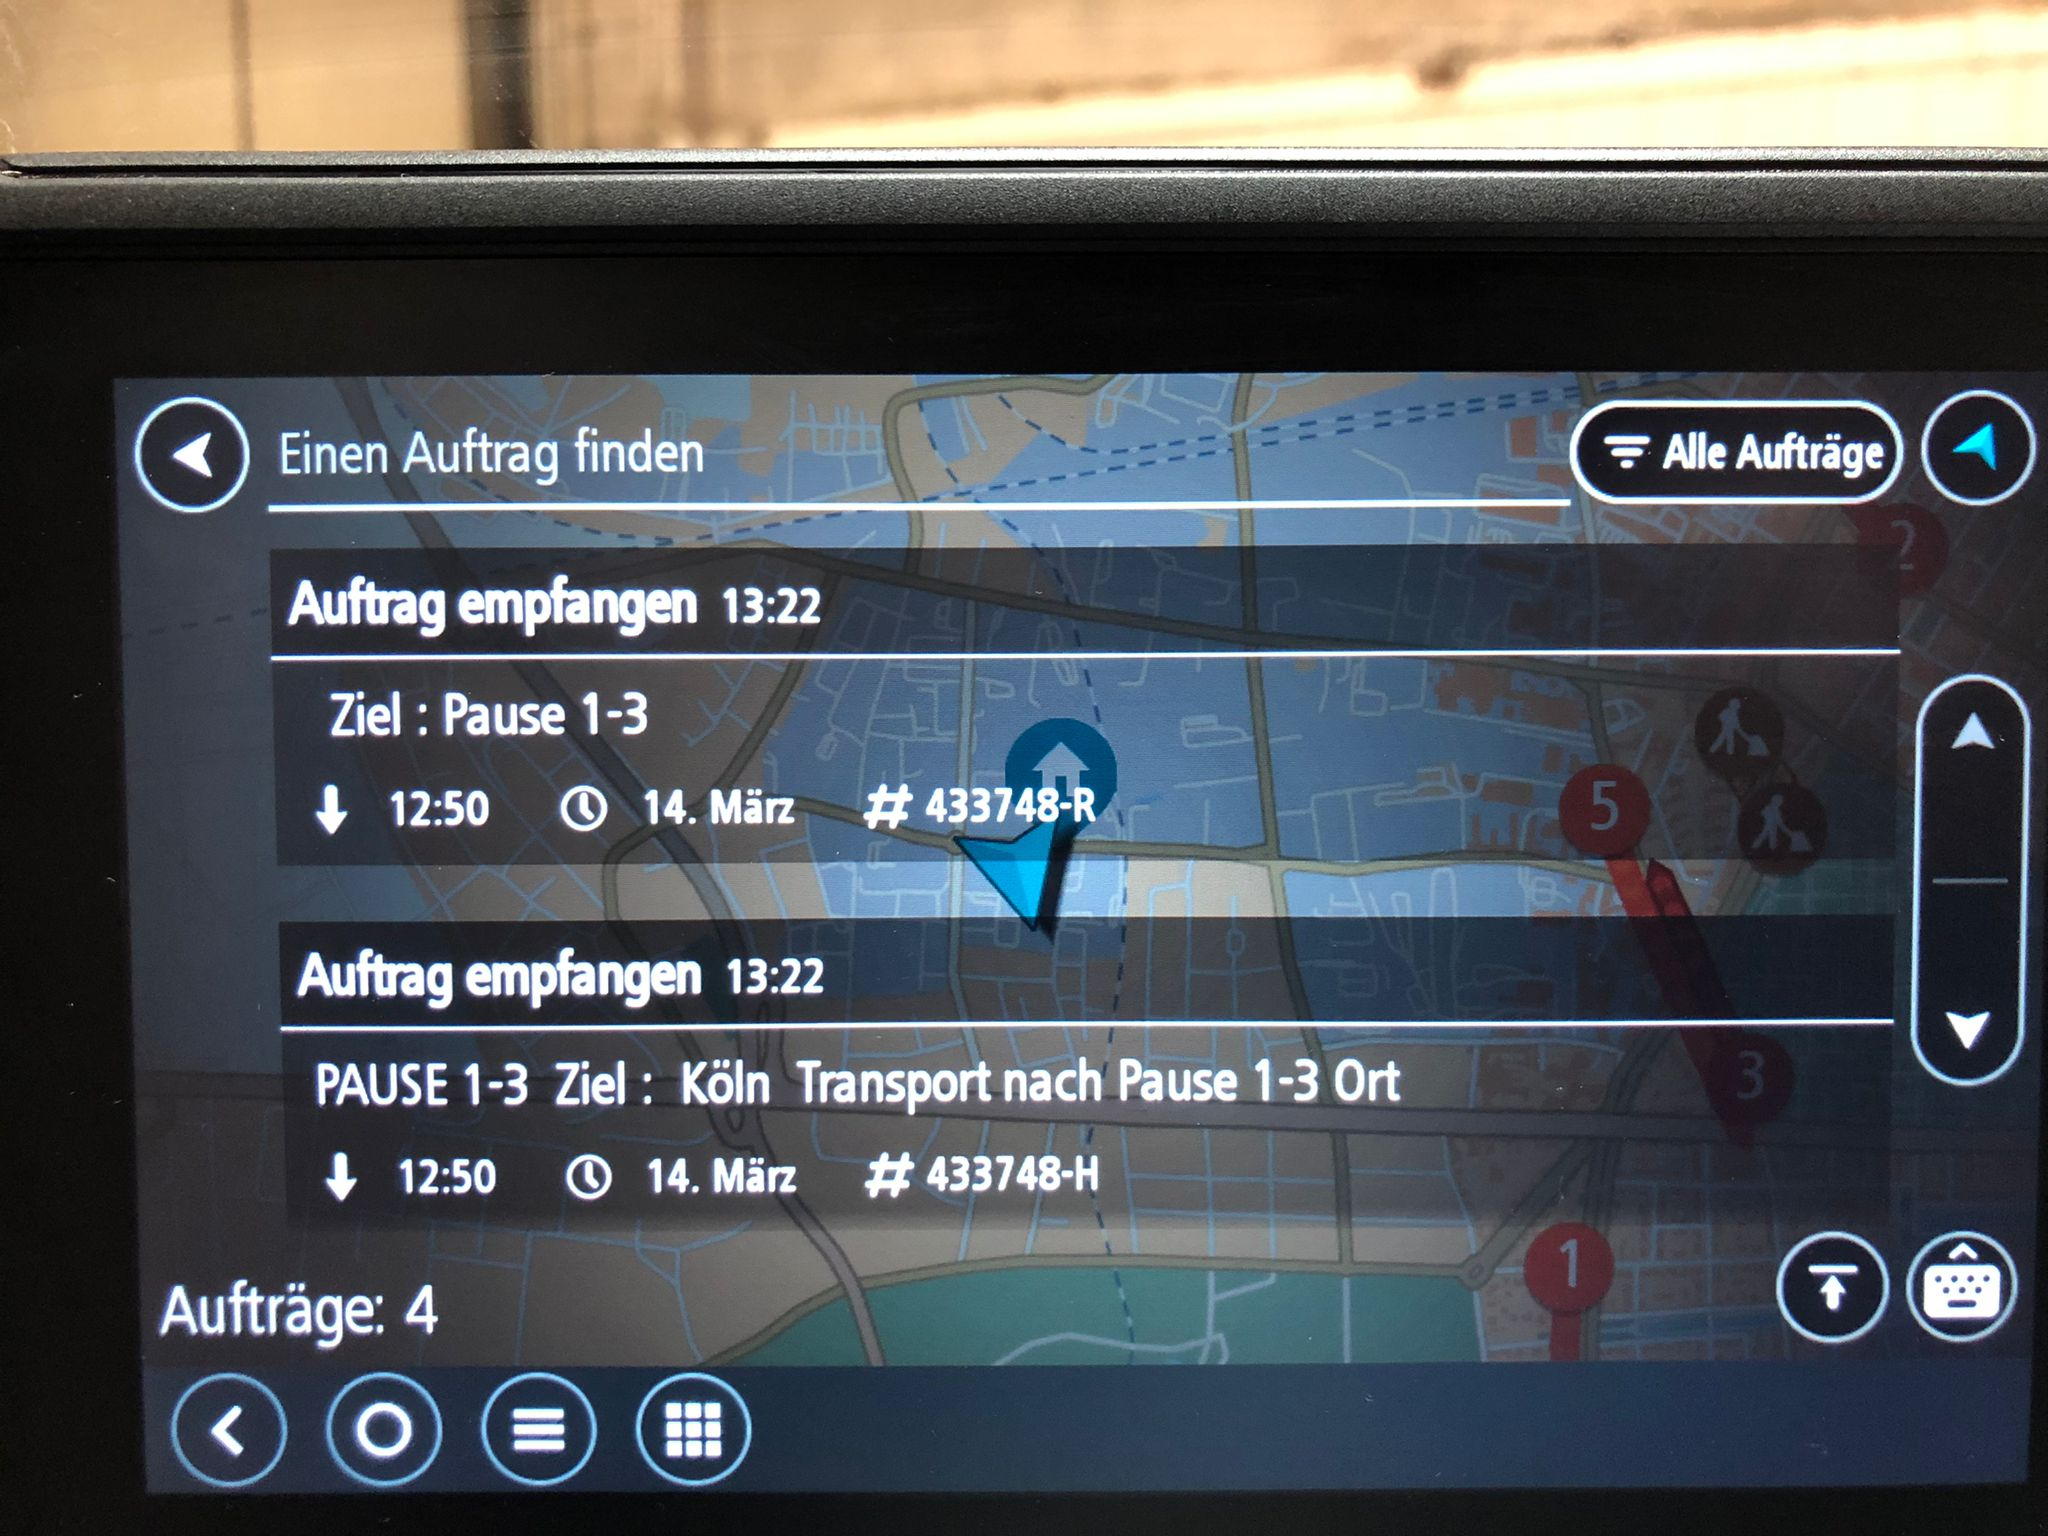
\includegraphics[width=5cm]{bilder/annahme.jpg}
            \caption{Einsatz Auswahl}
            \label{Auswahl}
        \end{center}
    \end{figure}
    
    \newpage
    \subsection{Aufträge akzeptieren}
    Im darauffolgenden Menü wird der Auftrag detailiert angezeigt. Dort findent ihr den Patienten Namen, "sitzend/liegend" und
    weitere Informationen zu dem Zustand des Patienten. Rechts unten findet ihr den Button Akzeptieren. Wenn ihr diesen drückt wird der Einsatz gestartet.
    \begin{figure}[h]
        \begin{center}
            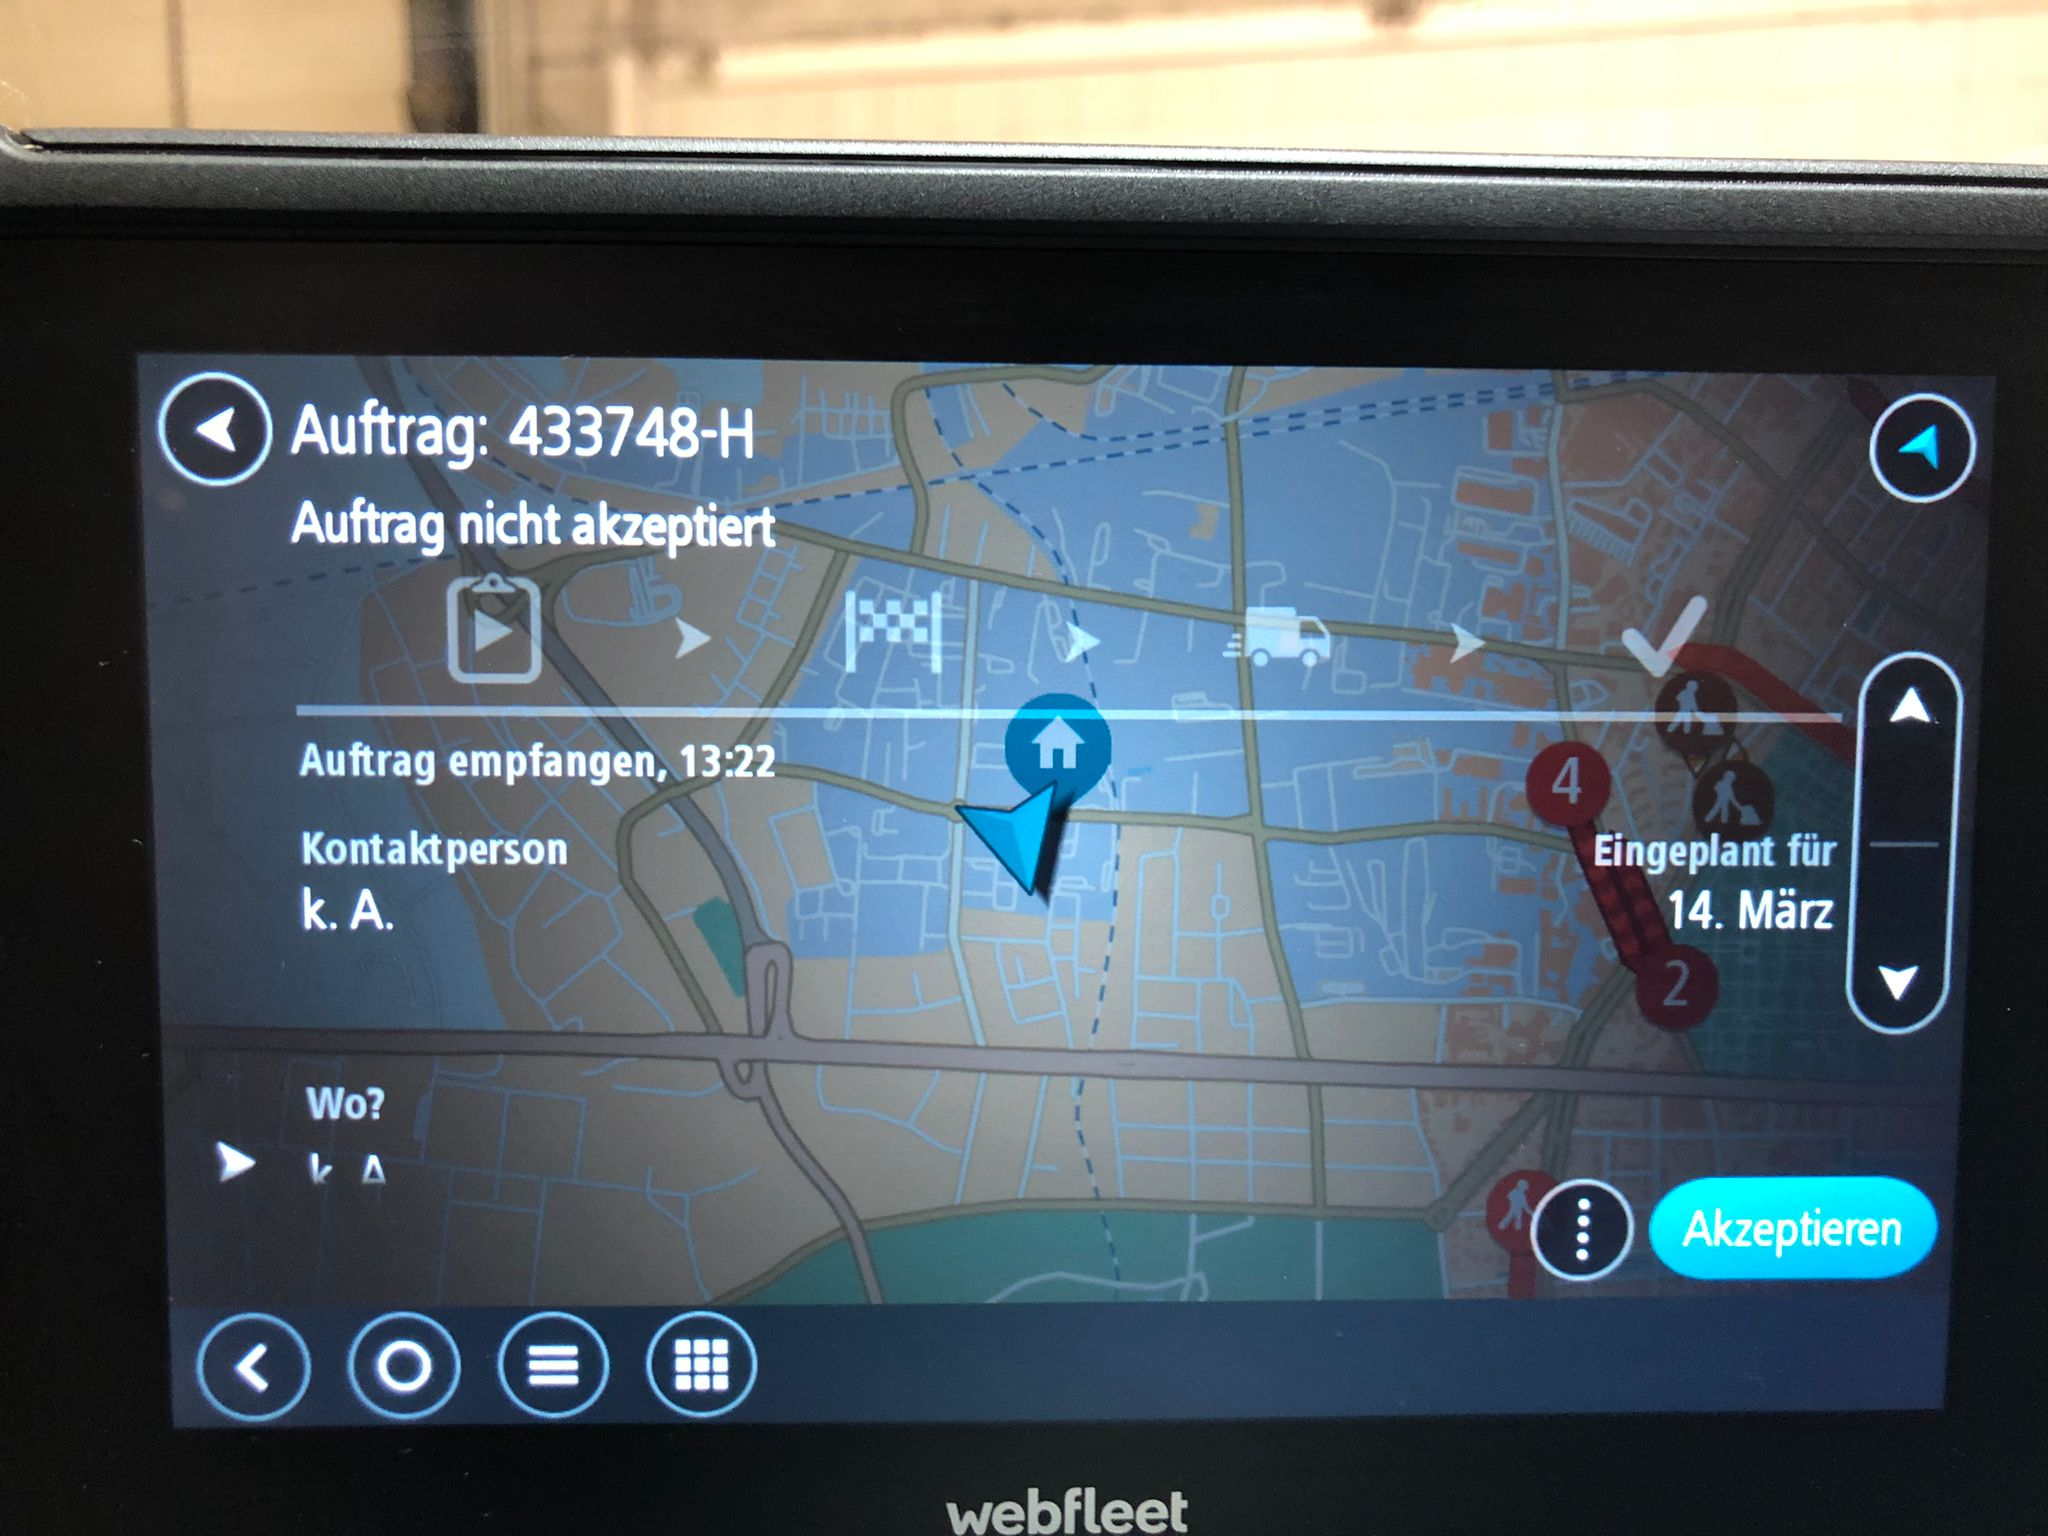
\includegraphics[width=5cm]{bilder/akzeptieren.jpg}
            \caption{Einsatz akzeptieren}
            \label{akzeptieren}
        \end{center}     
    \end{figure}

    \subsection{Status 3 Auftrag Beginnen}
    Nachdem ihr den Einsatz akzeptiert habt könnt ihr im nächsten Menü den Einsatz beginnen. Drückt ihr auf "Beginnen"
    so startet sich das Navi zum Einsatzort. Ihr befindet euch nun im Status 3 "Einsatz übernommen"
    \begin{figure}[h]
        \begin{center}
            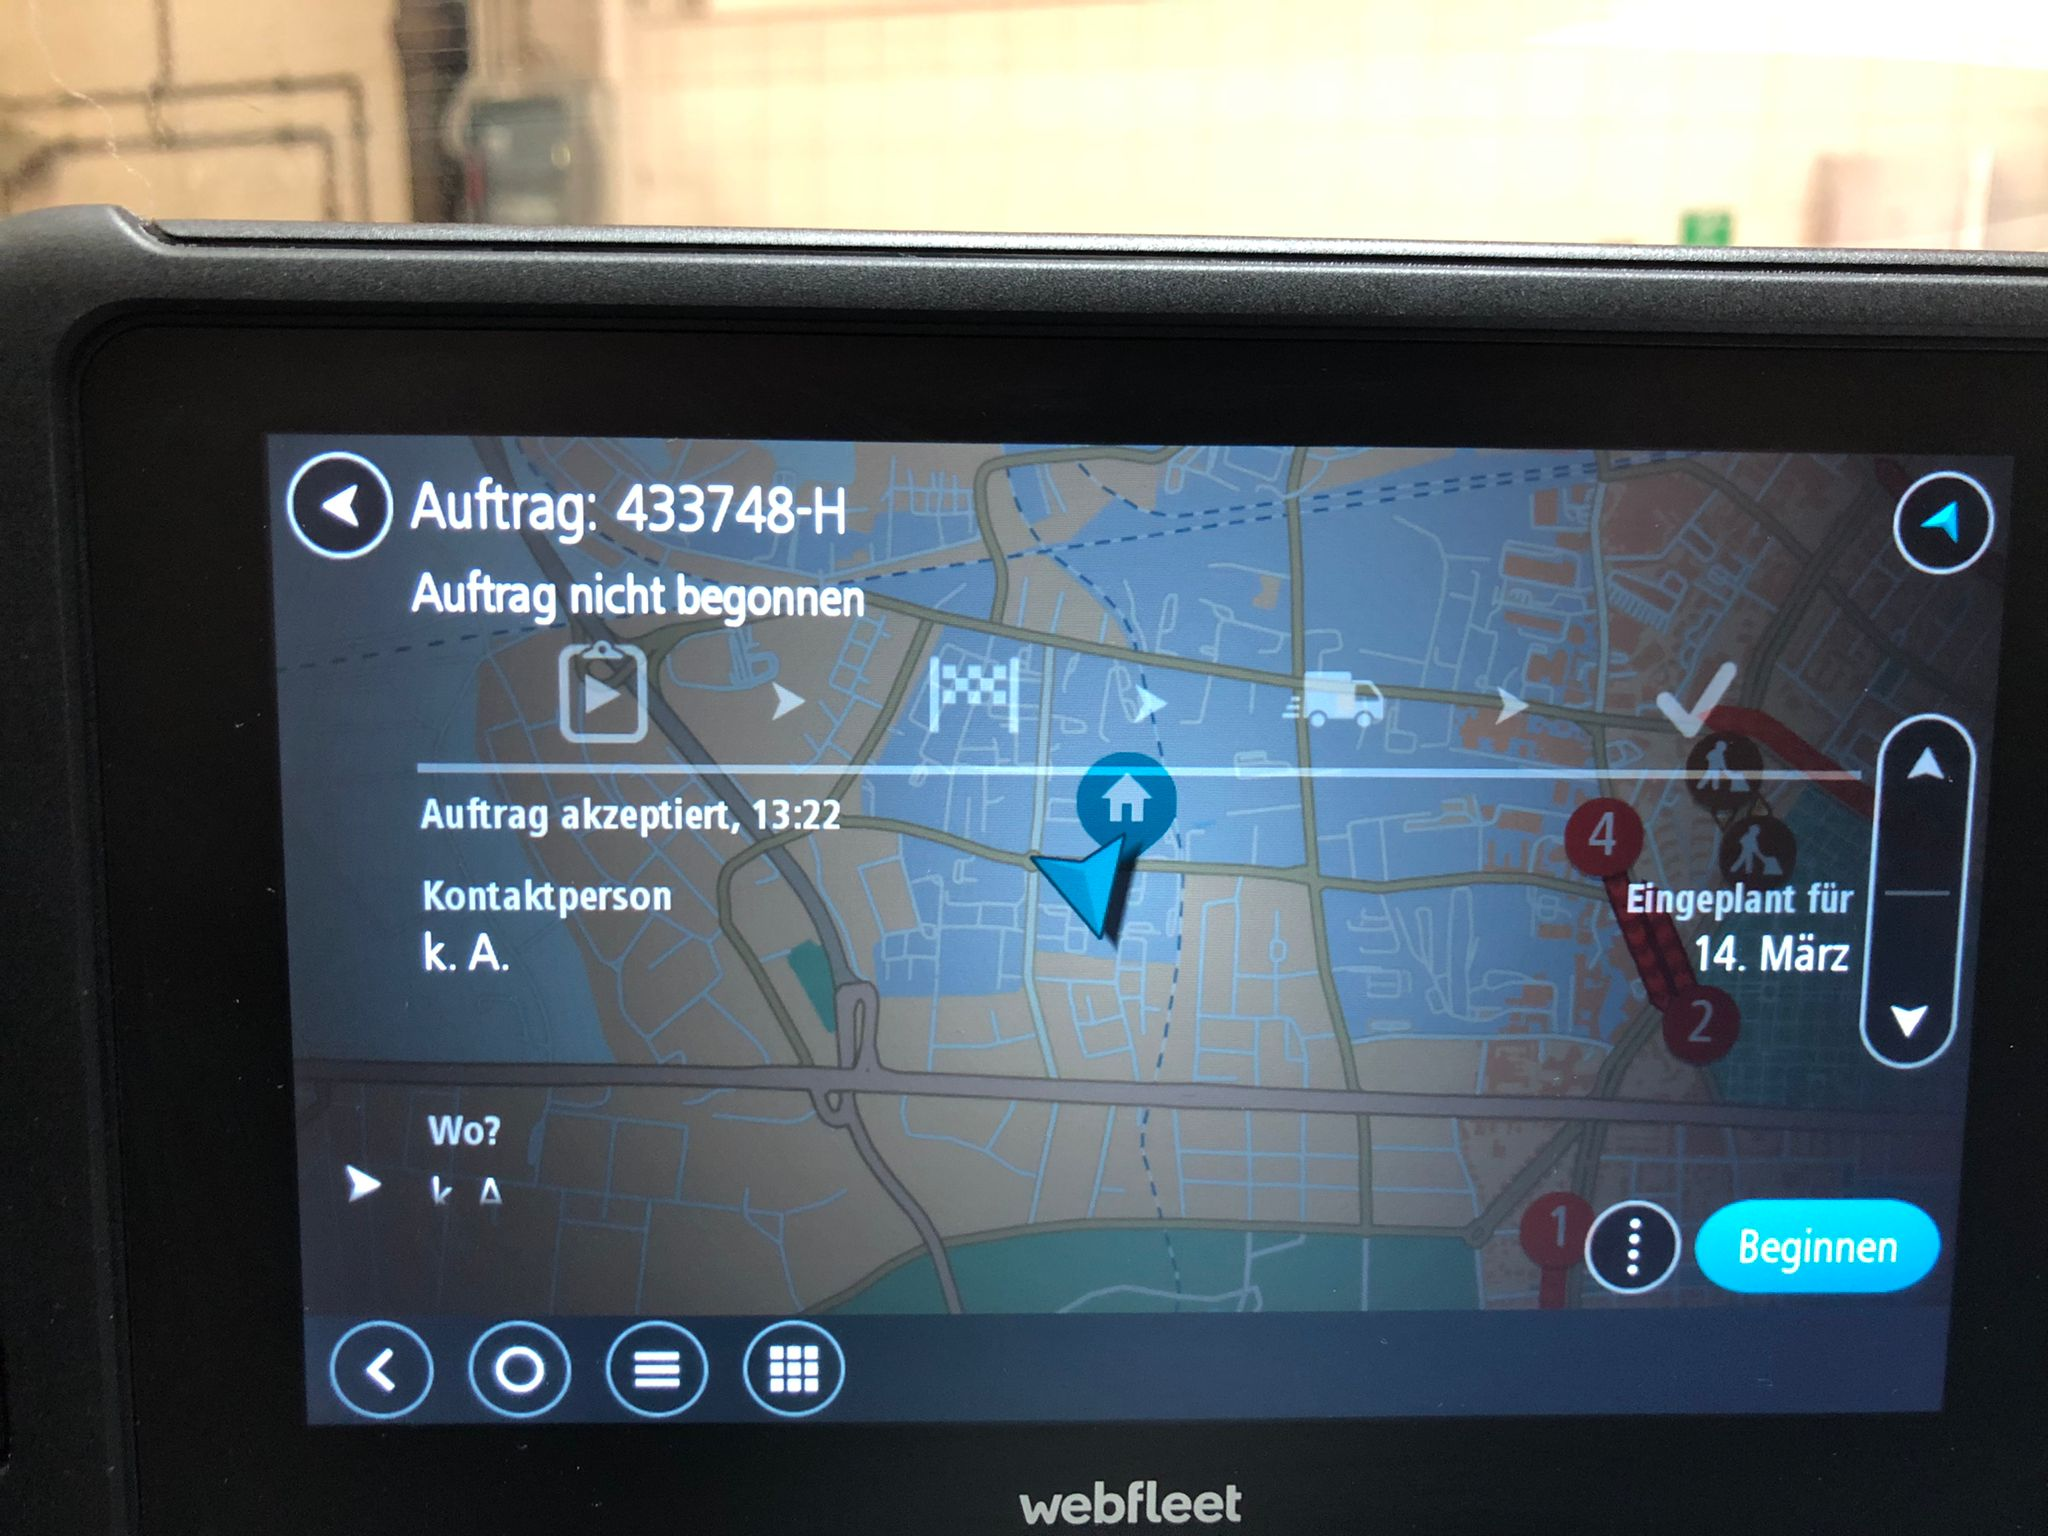
\includegraphics[width=5cm]{bilder/beginnen.jpg}
            \caption{Einsatz beginnen Status 3}
            \label{beginnen}
        \end{center}     
    \end{figure}
    
    \newpage
    \subsection{Einsatzort erreicht Status 4}
    Seid ihr am Einsatzort angekommen, könnt ihr im Einsatzmenü "Nächster Schritt" auswählen. Ihr befindet euch nun im Status 4 "Ankuft Einstatzstelle"
    \begin{figure}[h]
        \begin{center}
            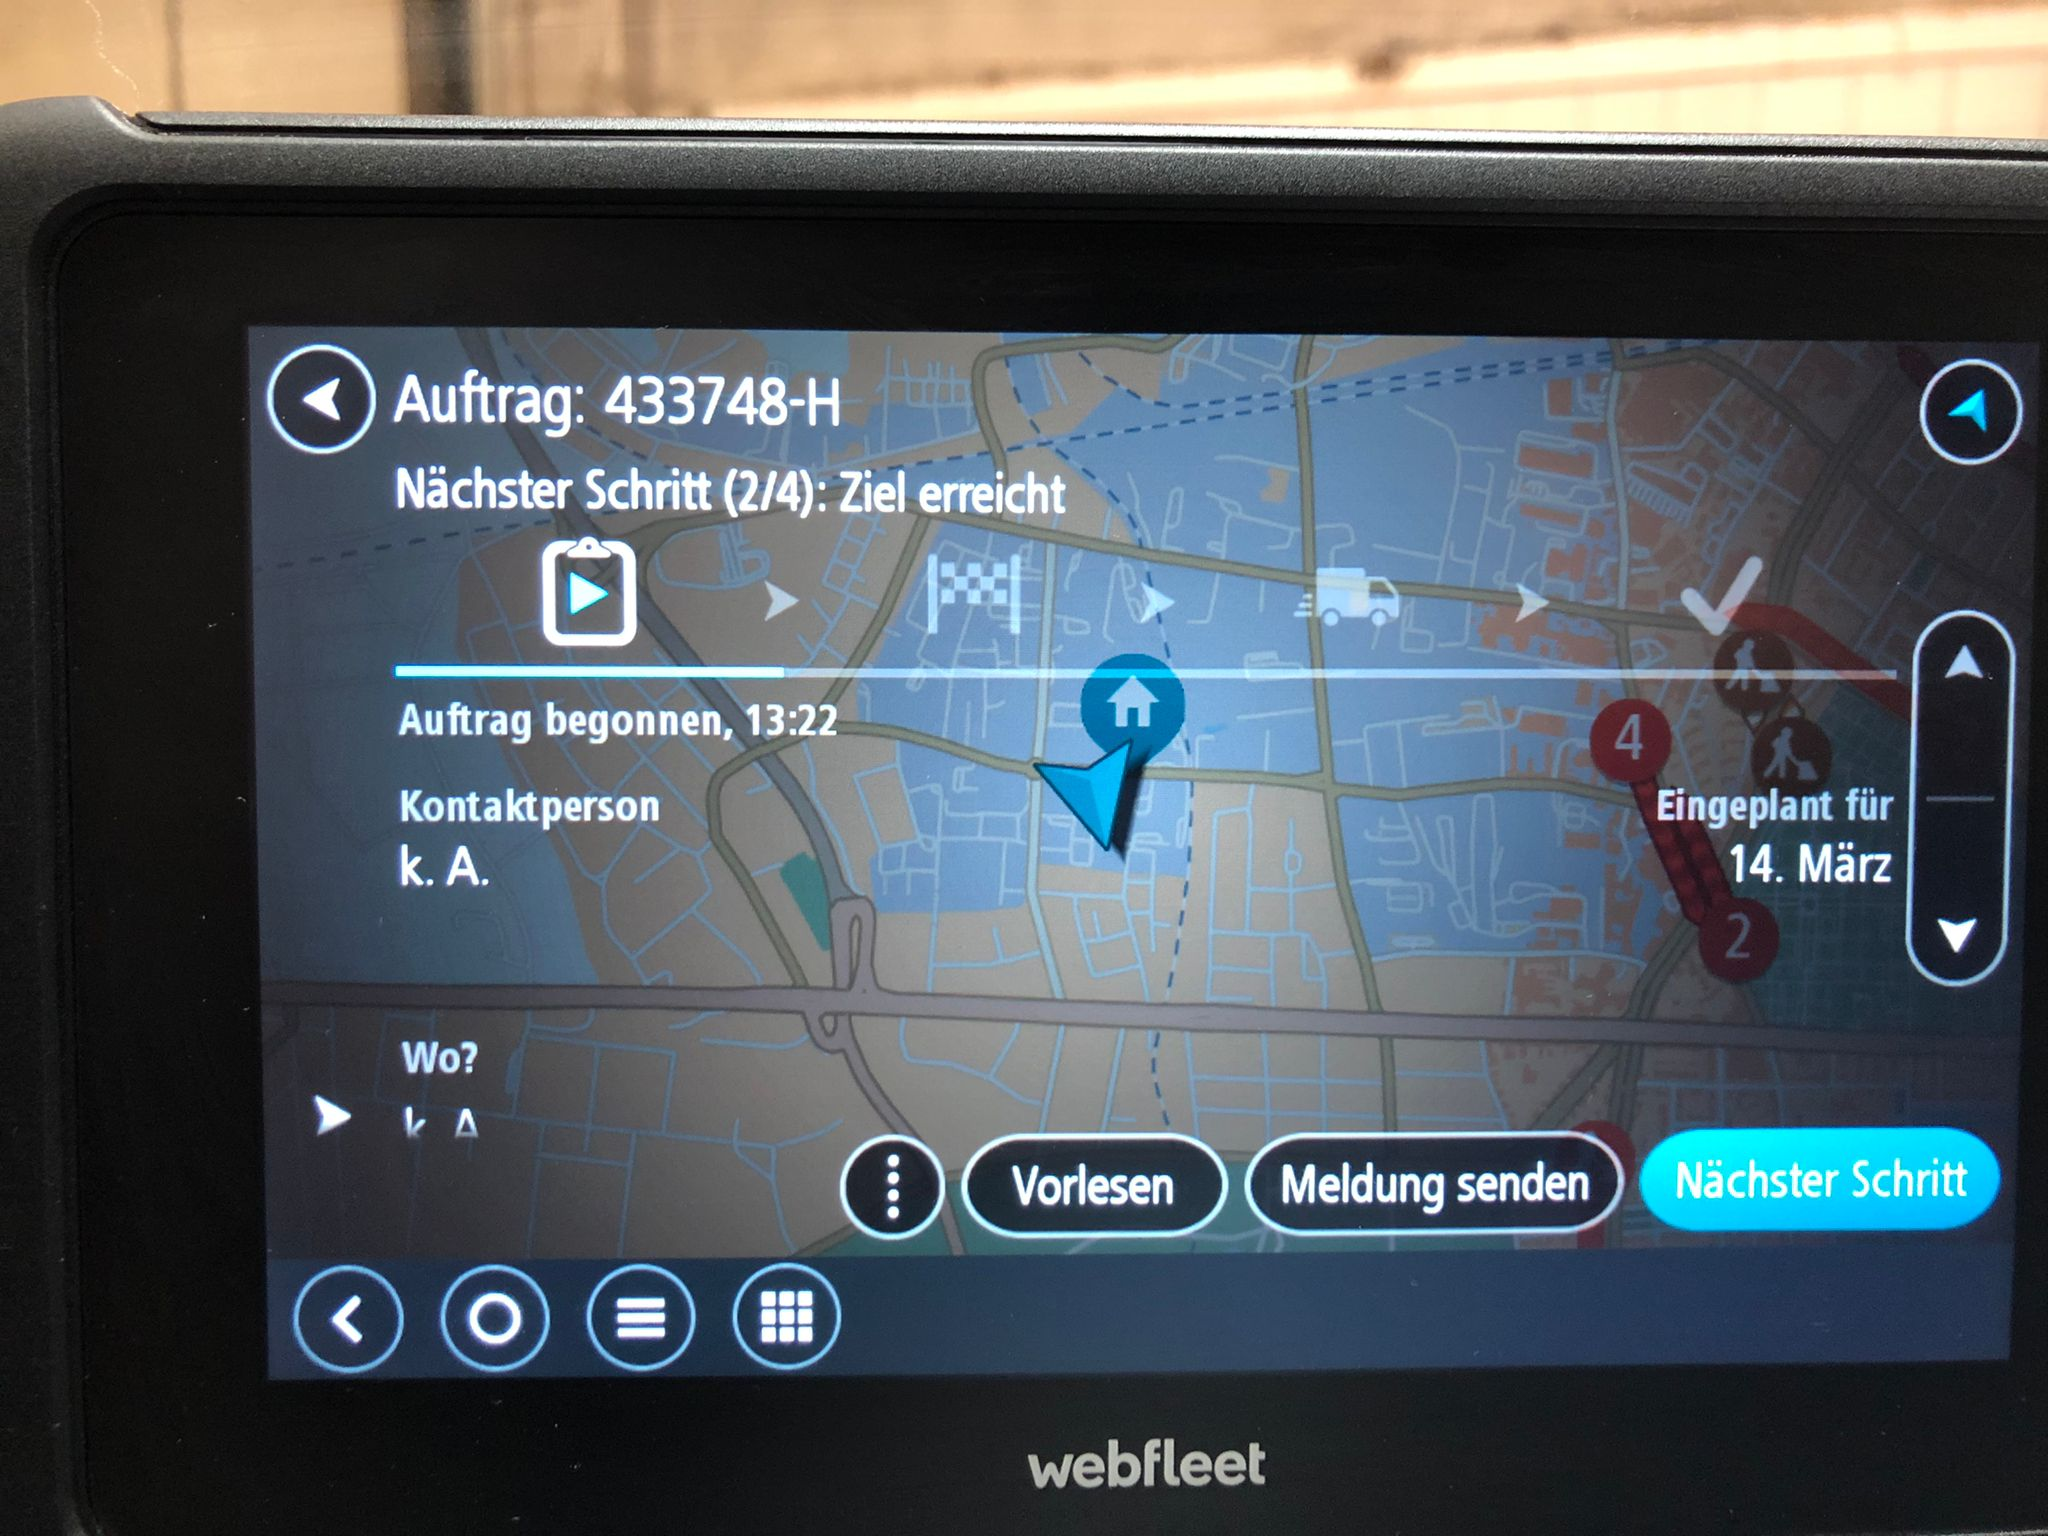
\includegraphics[width=5cm]{bilder/einsatzort.jpg}
            \caption{Ankunft Einsatzstelle Status 4}
            \label{ankunft Einsatzstelle}
        \end{center} 
    \end{figure}
    
    \subsection{Patient aufgenommen Status 7}
    Ist der Patient Aufgenommen wählt nun wieder "Nächster Schritt". Euch wird die Route zum Zielort angezeigt.
    Ihr befindet euch nun im Status 7 "Aufgenommen"
    \begin{figure}[h]
        \begin{center}
            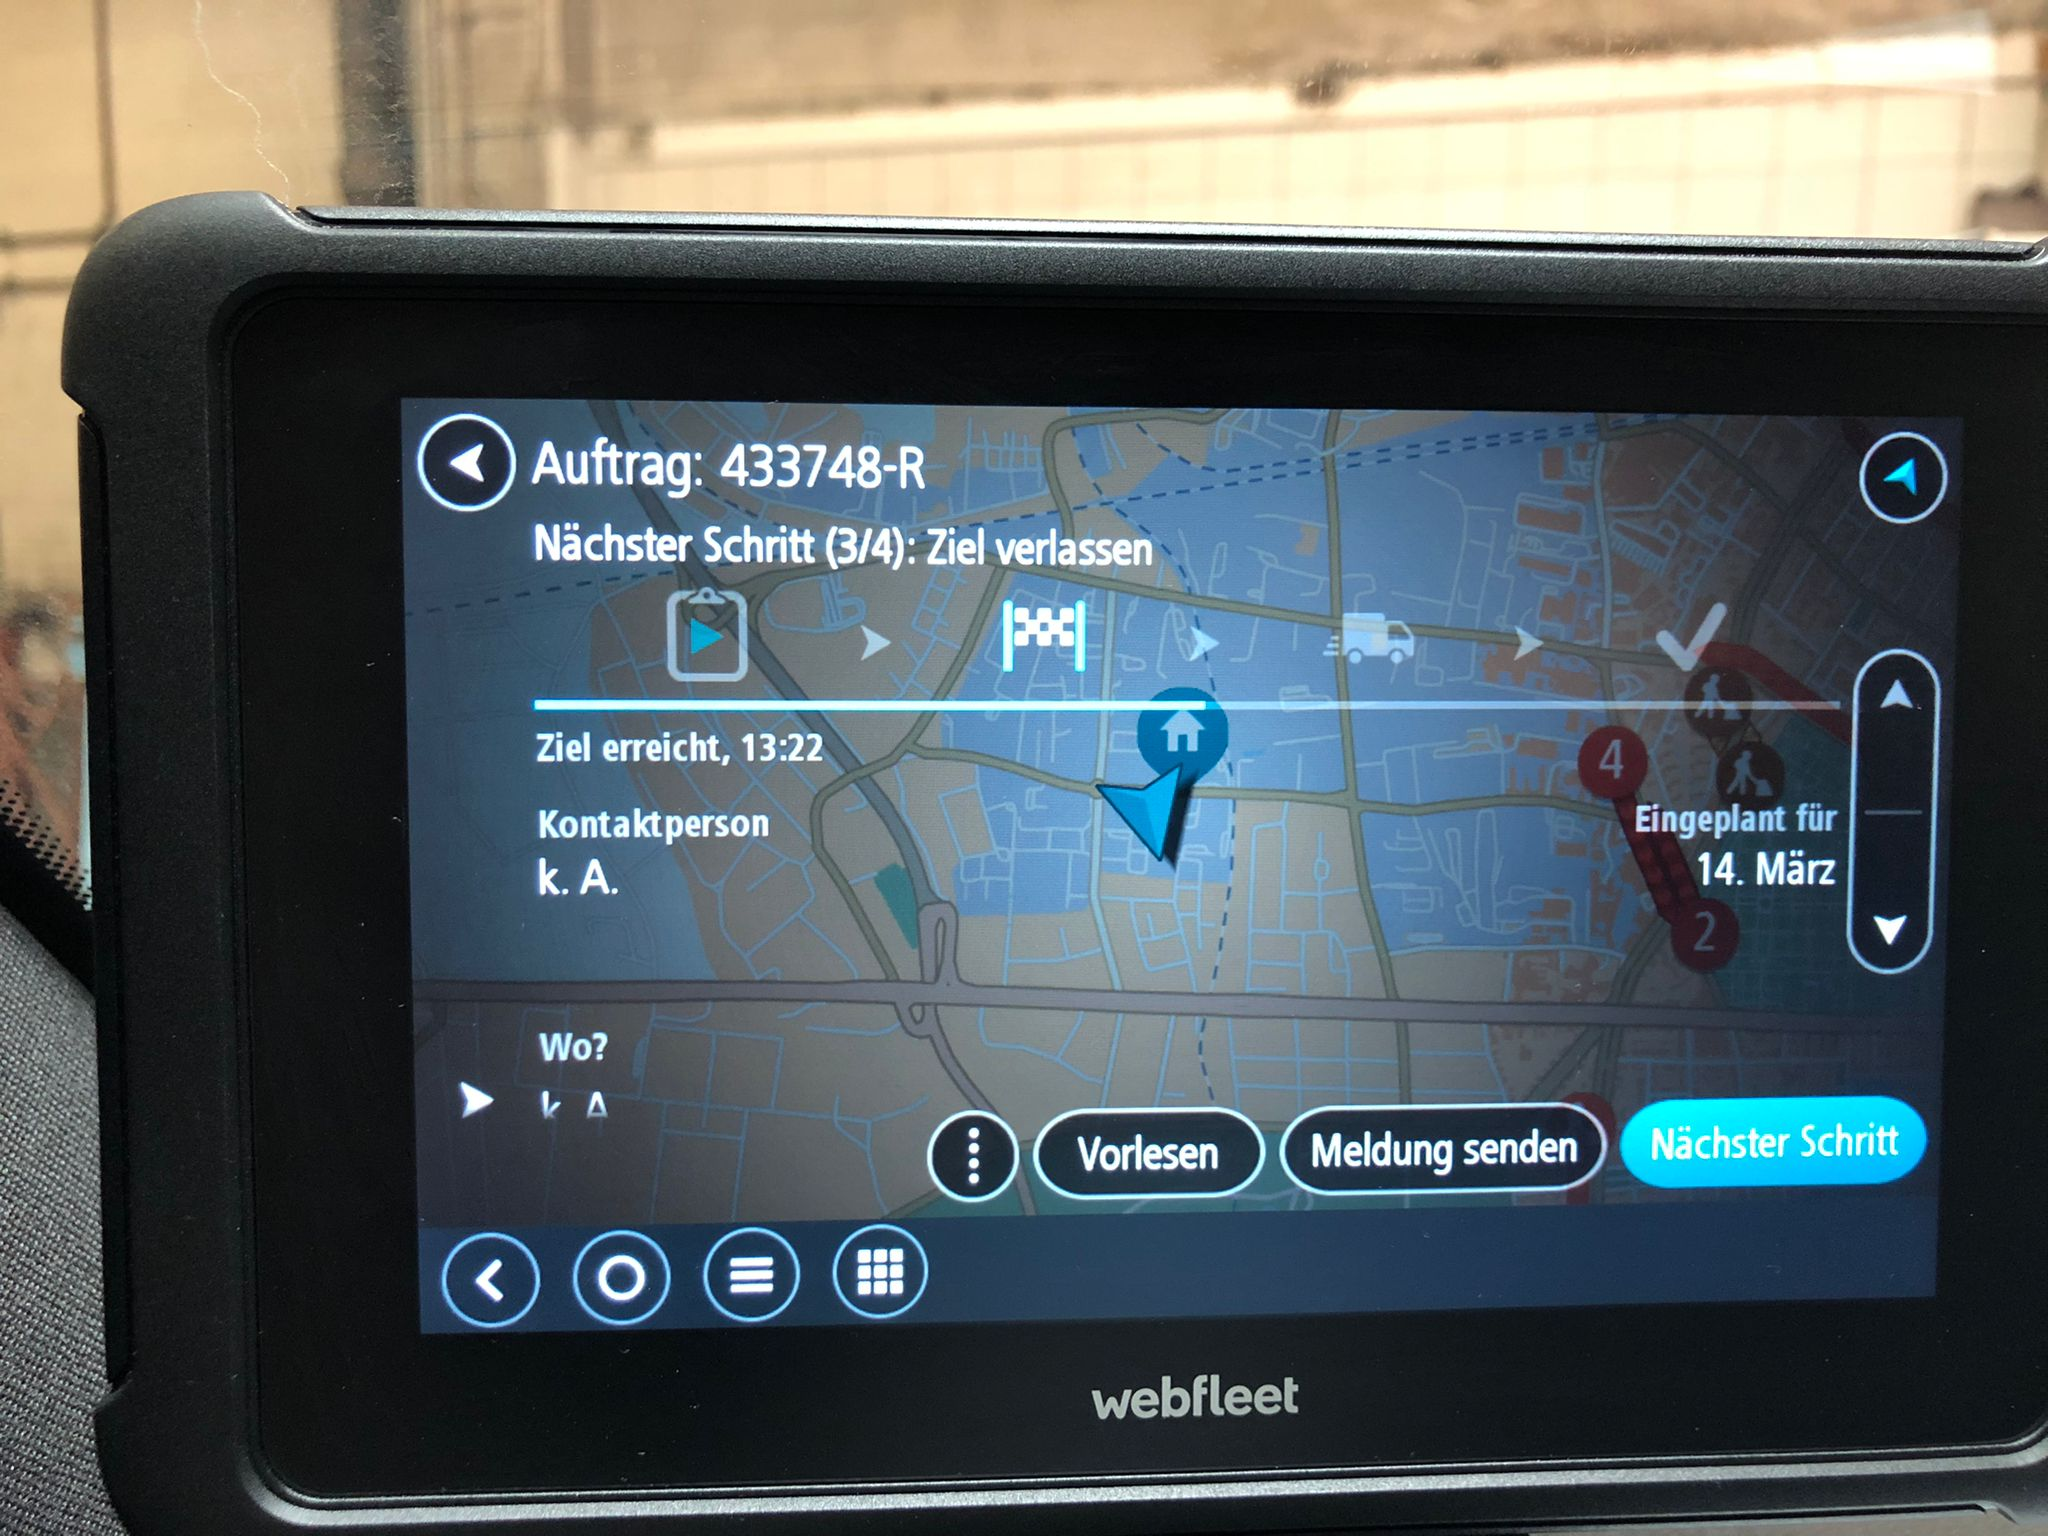
\includegraphics[width=5cm]{bilder/aufgenommen.jpg}
            \caption{Patient aufgenommen Status 7}
            \label{Patient aufgenommen}
        \end{center} 
    \end{figure}

    \newpage
    \subsection{Zielort erreicht Status 8}
    Sobalt ihr am Zielort angekommen seit wählt ihr wieder "Nächster Schritt". Ihr befindet euch nun im Status 8 "Am Zielort angekommen".
    Im idealfall wird euch die Leitstelle nun den Folgeauftrag schicken oder euch Infos per Messenger schicken.
    \begin{figure}[h]
        \begin{center}
            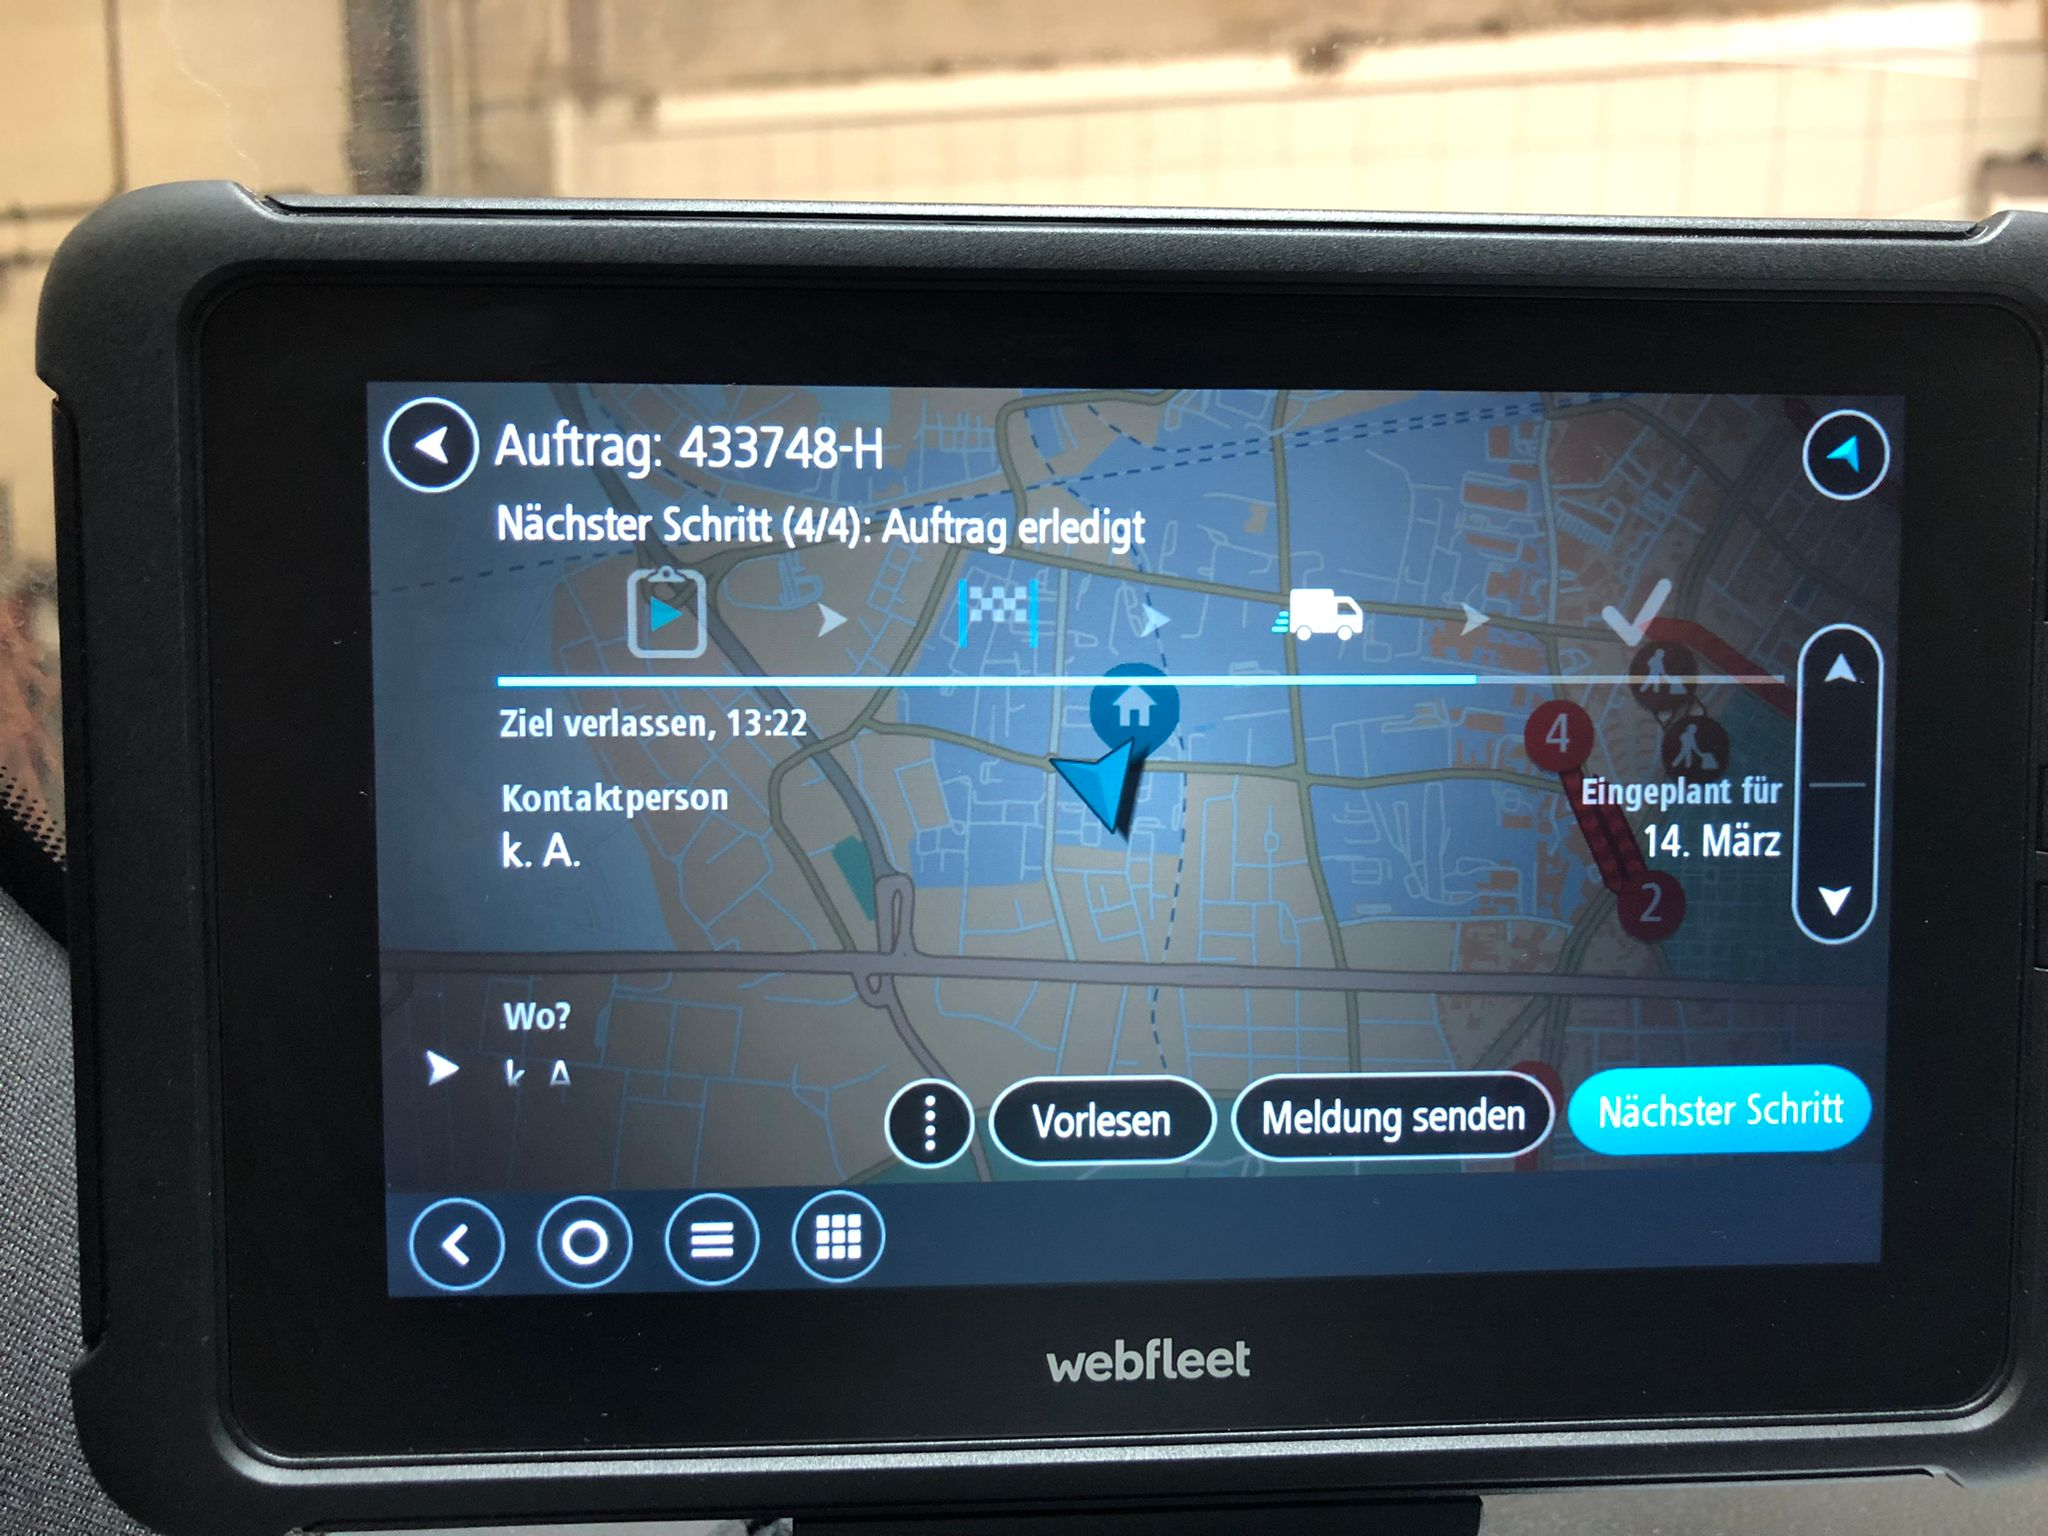
\includegraphics[width=5cm]{bilder/angekommen.jpg}
            \caption{Am Ziel angekommen Status 8}
            \label{Ziel}
        \end{center} 
    \end{figure}

    \subsection{Einsatz beenden Status 1}
    Ist der Patient am Zielort übergeben und der KTW wieder einsatzbereit wählt ihr wieder "Nächster Schritt.
    Ihr befindet euch nun wieder im Status 1 "Frei" bzw. "Frei Wache". Wenn die Einsatzdokumentation abgeschlossen ist 
    könnt ihr den Einsatz mit einem druck auf den Button "Löschen" von eurem Navi entfernen. Dies könnt ihr natürlich 
    auch gesammelt vor Feierabend machen. 
    \begin{figure}[h]
        \begin{center}
            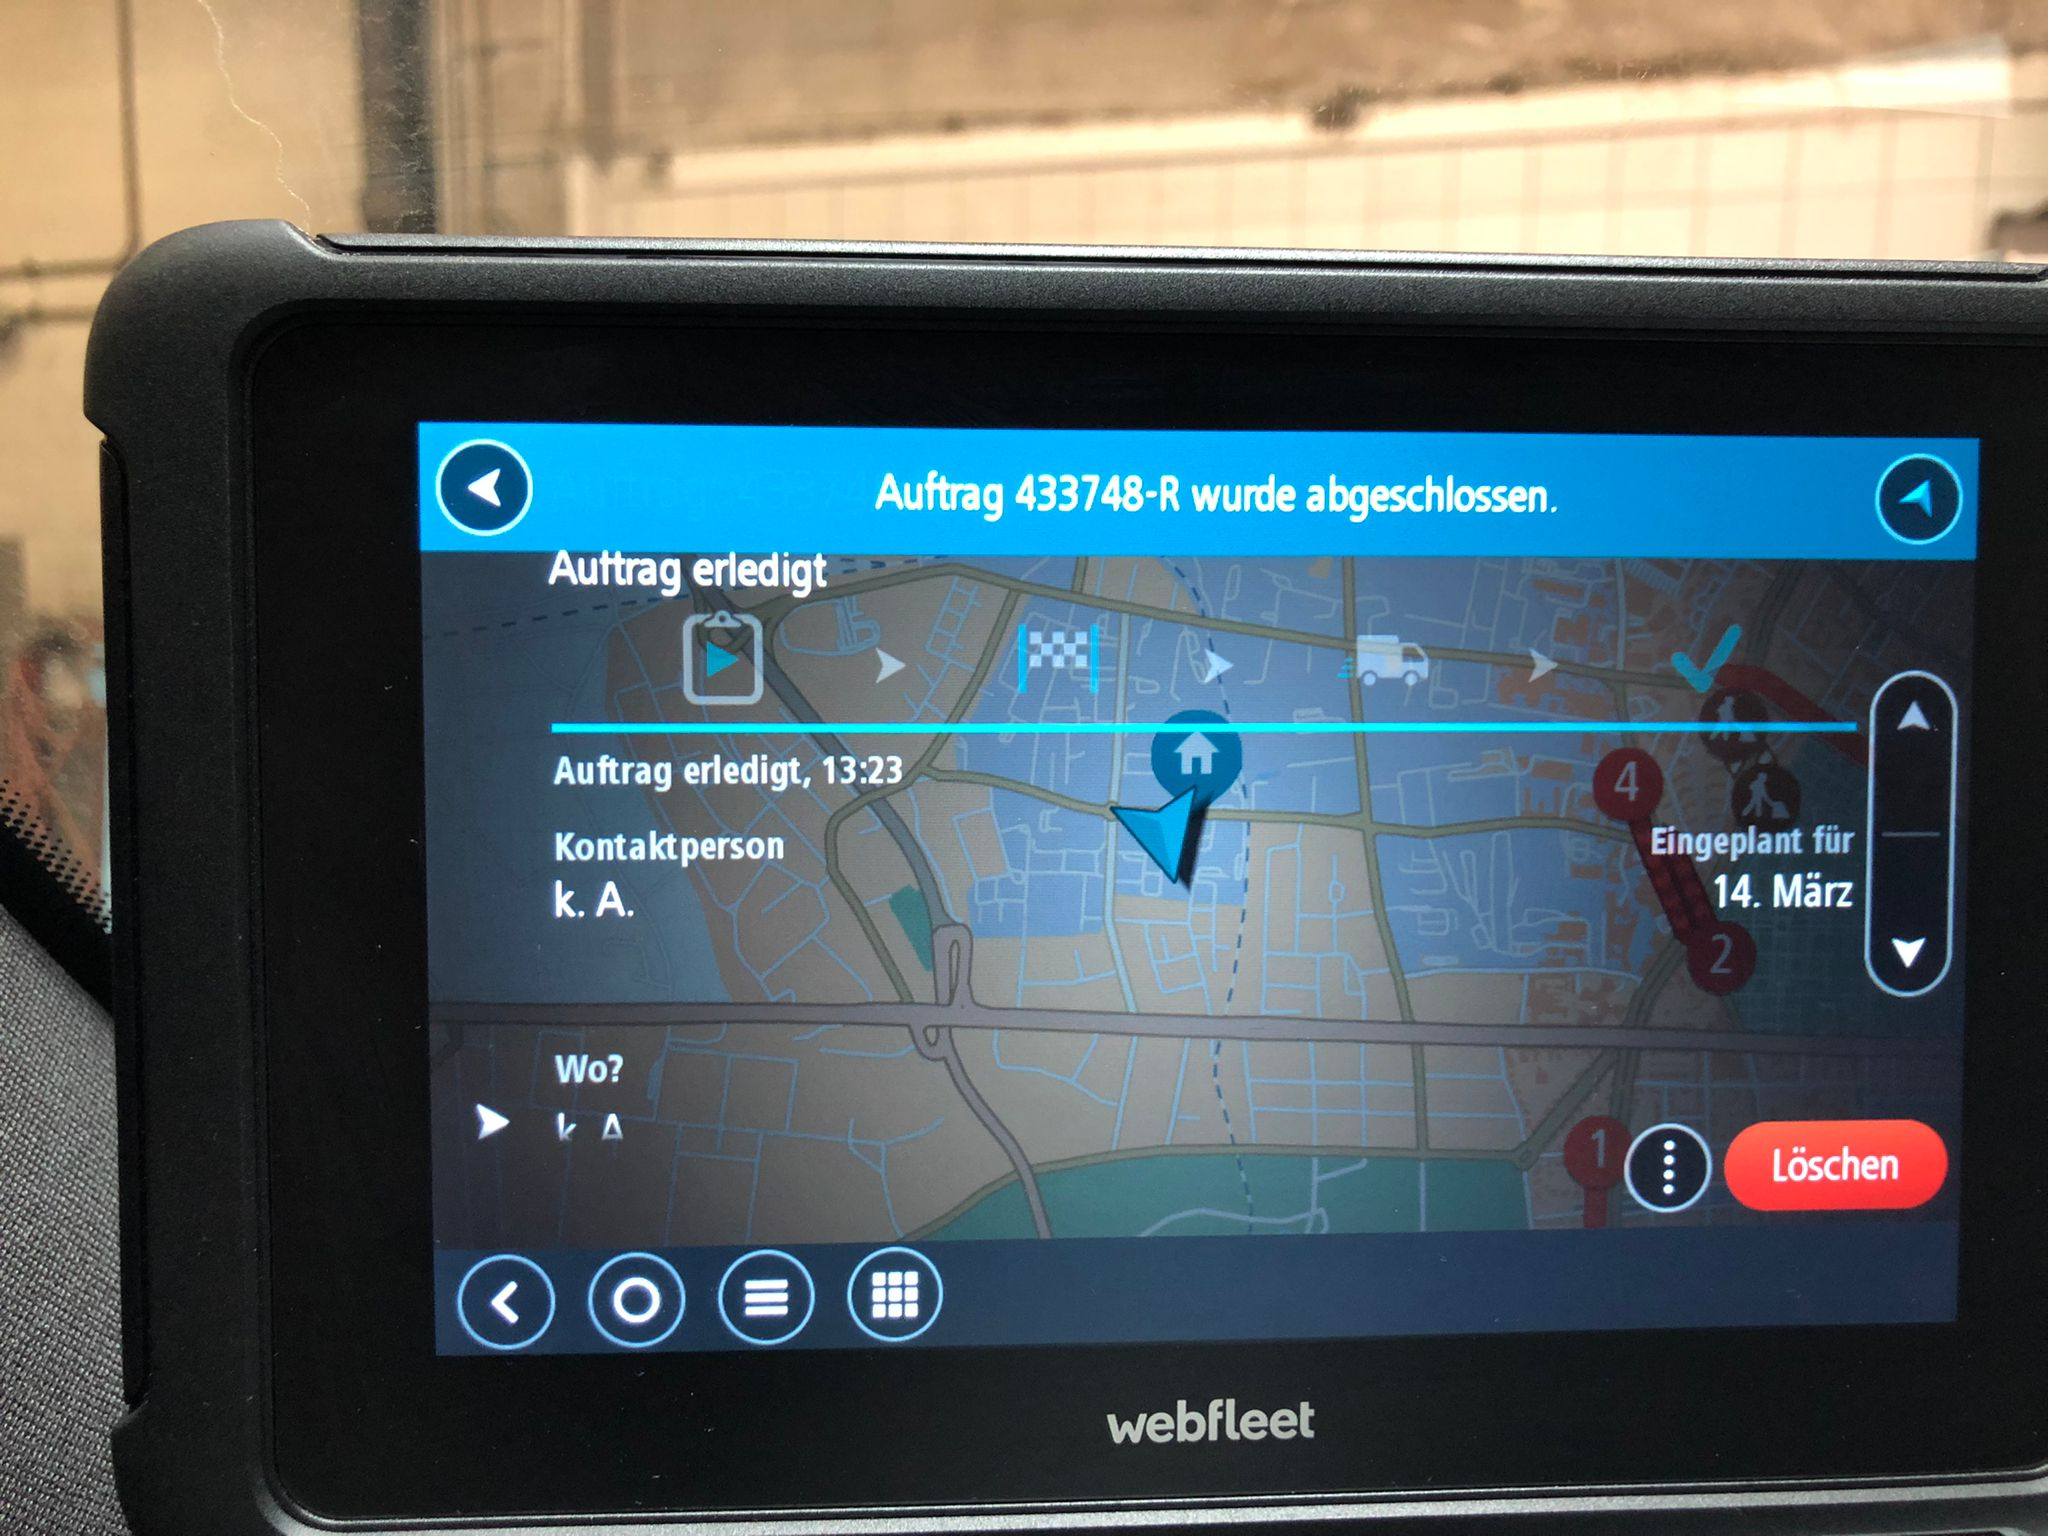
\includegraphics[width=5cm]{bilder/beenden.jpg}
            \caption{Einsatz beenden Status 1}
            \label{Beenden}
        \end{center} 
    \end{figure}
    \newline Achtet bitte darauf das am Ende der Schicht alle Einsättze von dem Navi gelöscht wurden. Damit die folgebesatzung
    zur nächsten Schicht dies nicht für euch tun muss.

    \newpage
    \section{Manuelle Statigabe}
    Eine weitere Möglichket Stati zu geben ist die manuelle Statigabe. Dies empfiehlt sich z.B. wenn ihr
    aus versehen einen Stati zu weit gegeben habt oder es Probleme gibt die ihr nicht alleine lösen 
    könnt oder wollt.Leider ist das Menü zur Statigabe etwas versteckt.
    Desshalb gehen wir die einzelnen Schritte im detail durch.
    

    \subsection{Schritt 1 Smiley}
    Im Hauptmenü von Webfleet seht ihr am linken unteren Rand ein Smiley Symbol. Wählt dieses um ins nächste
    Menü zu gelangen.
    \begin{figure}[h]
        \begin{center}
            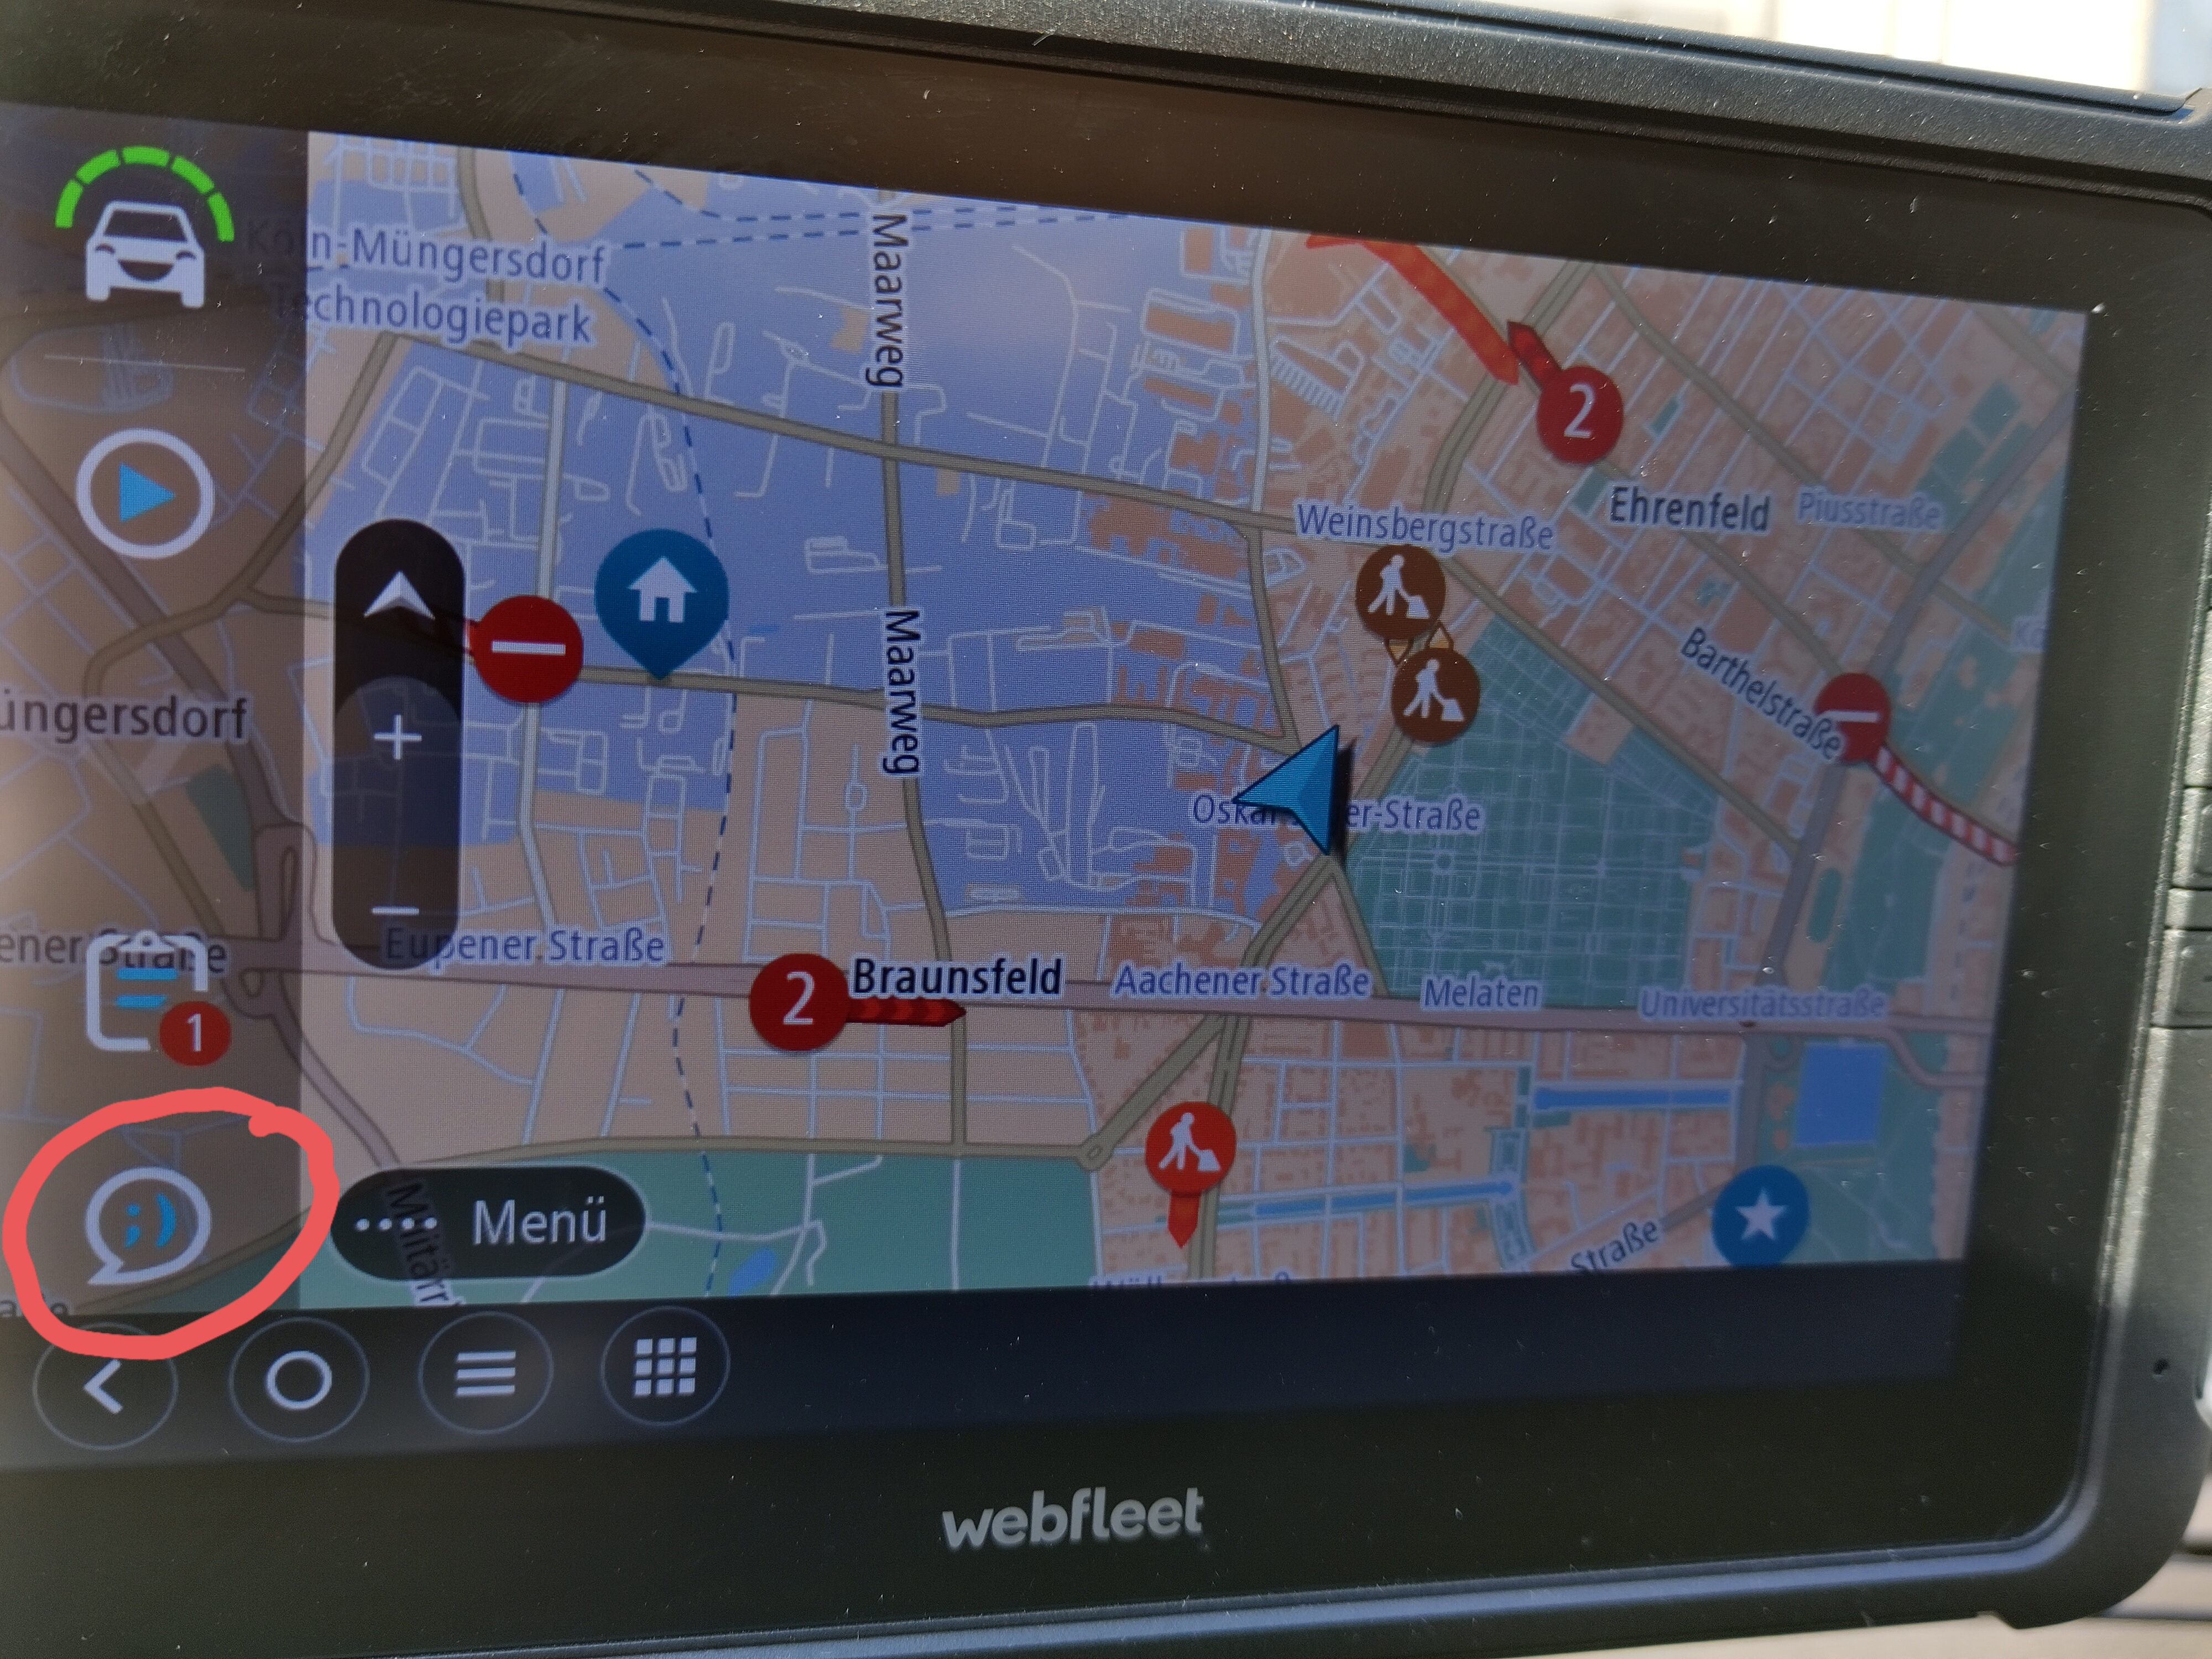
\includegraphics[width=5cm]{bilder/Schritt1.jpg}
            \caption{Schritt1 Smiley}
            \label{Smiley}
        \end{center} 
    \end{figure}

    \subsection{Schritt 2 Neue Meldung}
    In diesm Menü wählt ihr "Neue Meldung" um ins nächste Menü zu gelangen.
    \begin{figure}[h]
        \begin{center}
            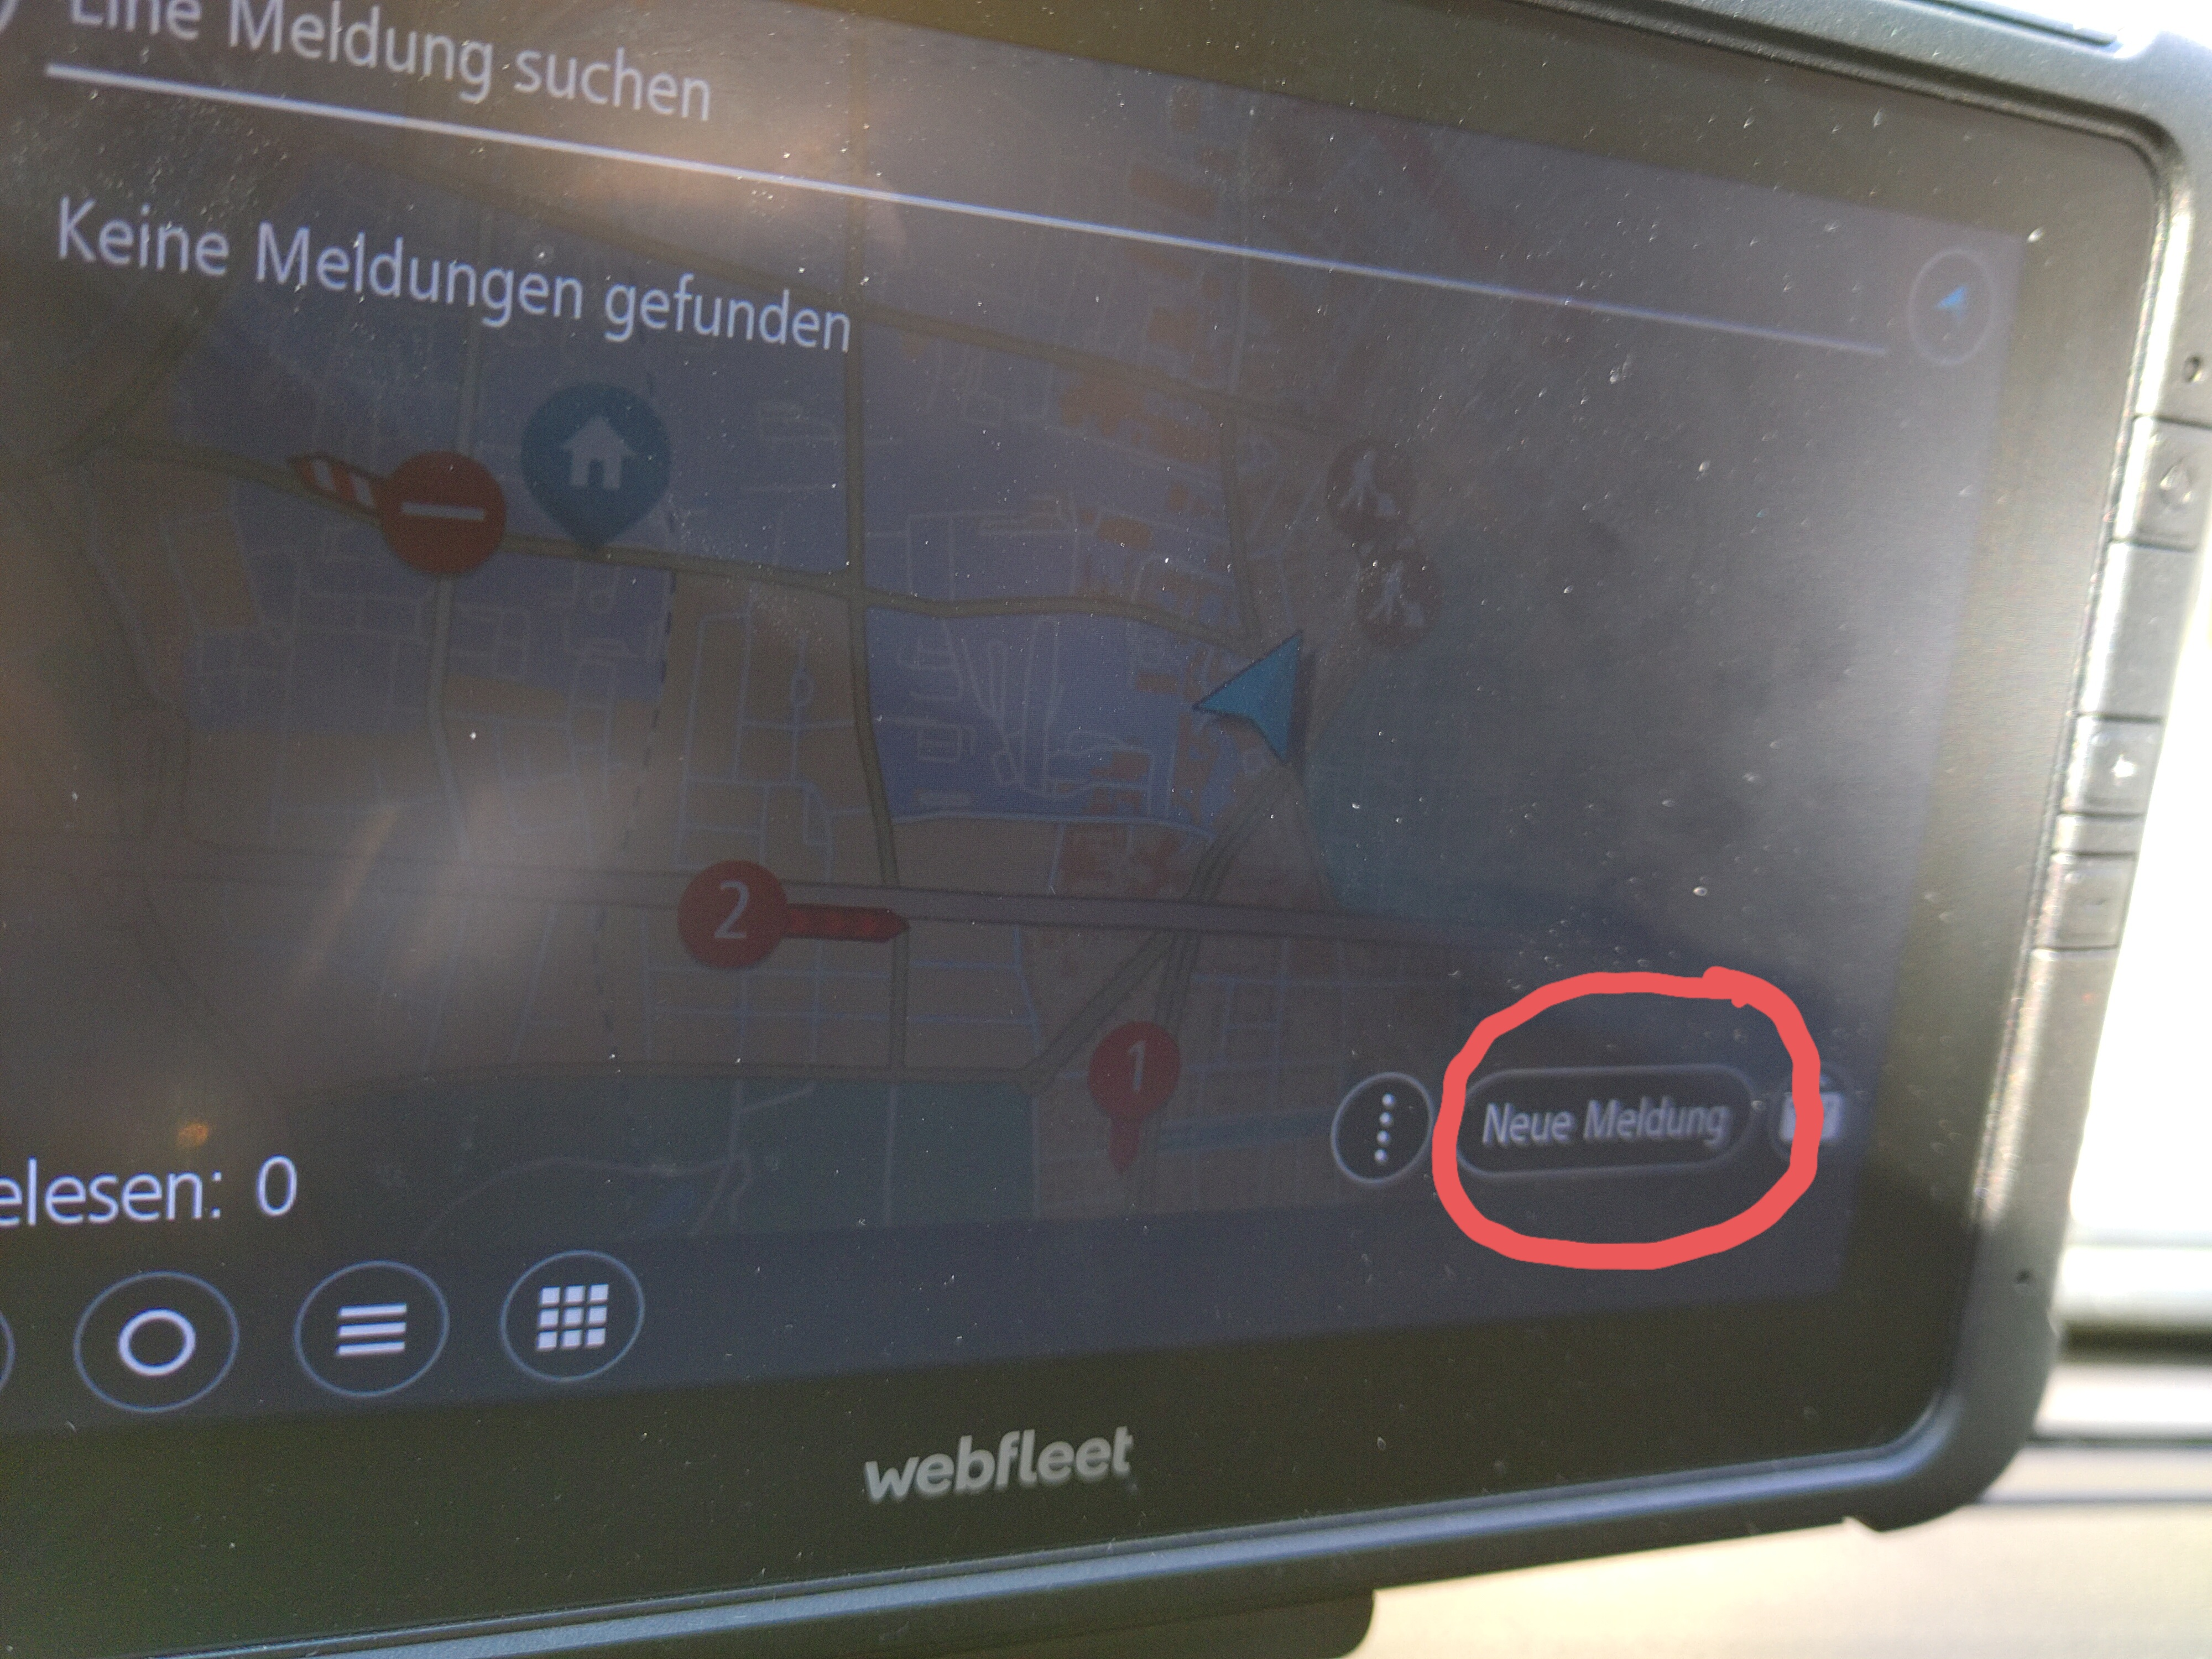
\includegraphics[width=5cm]{bilder/Schritt2.jpg}
            \caption{Schritt 2 Neue Meldung}
            \label{Neue Meldung}
        \end{center} 
    \end{figure}

    \newpage
    \subsection{Schritt 3 Vorlage}
    In diesem Menü wählt ihr "Vorlagen" um zum nächsten Menü zu gelangen.
    \begin{figure}[h]
        \begin{center}
            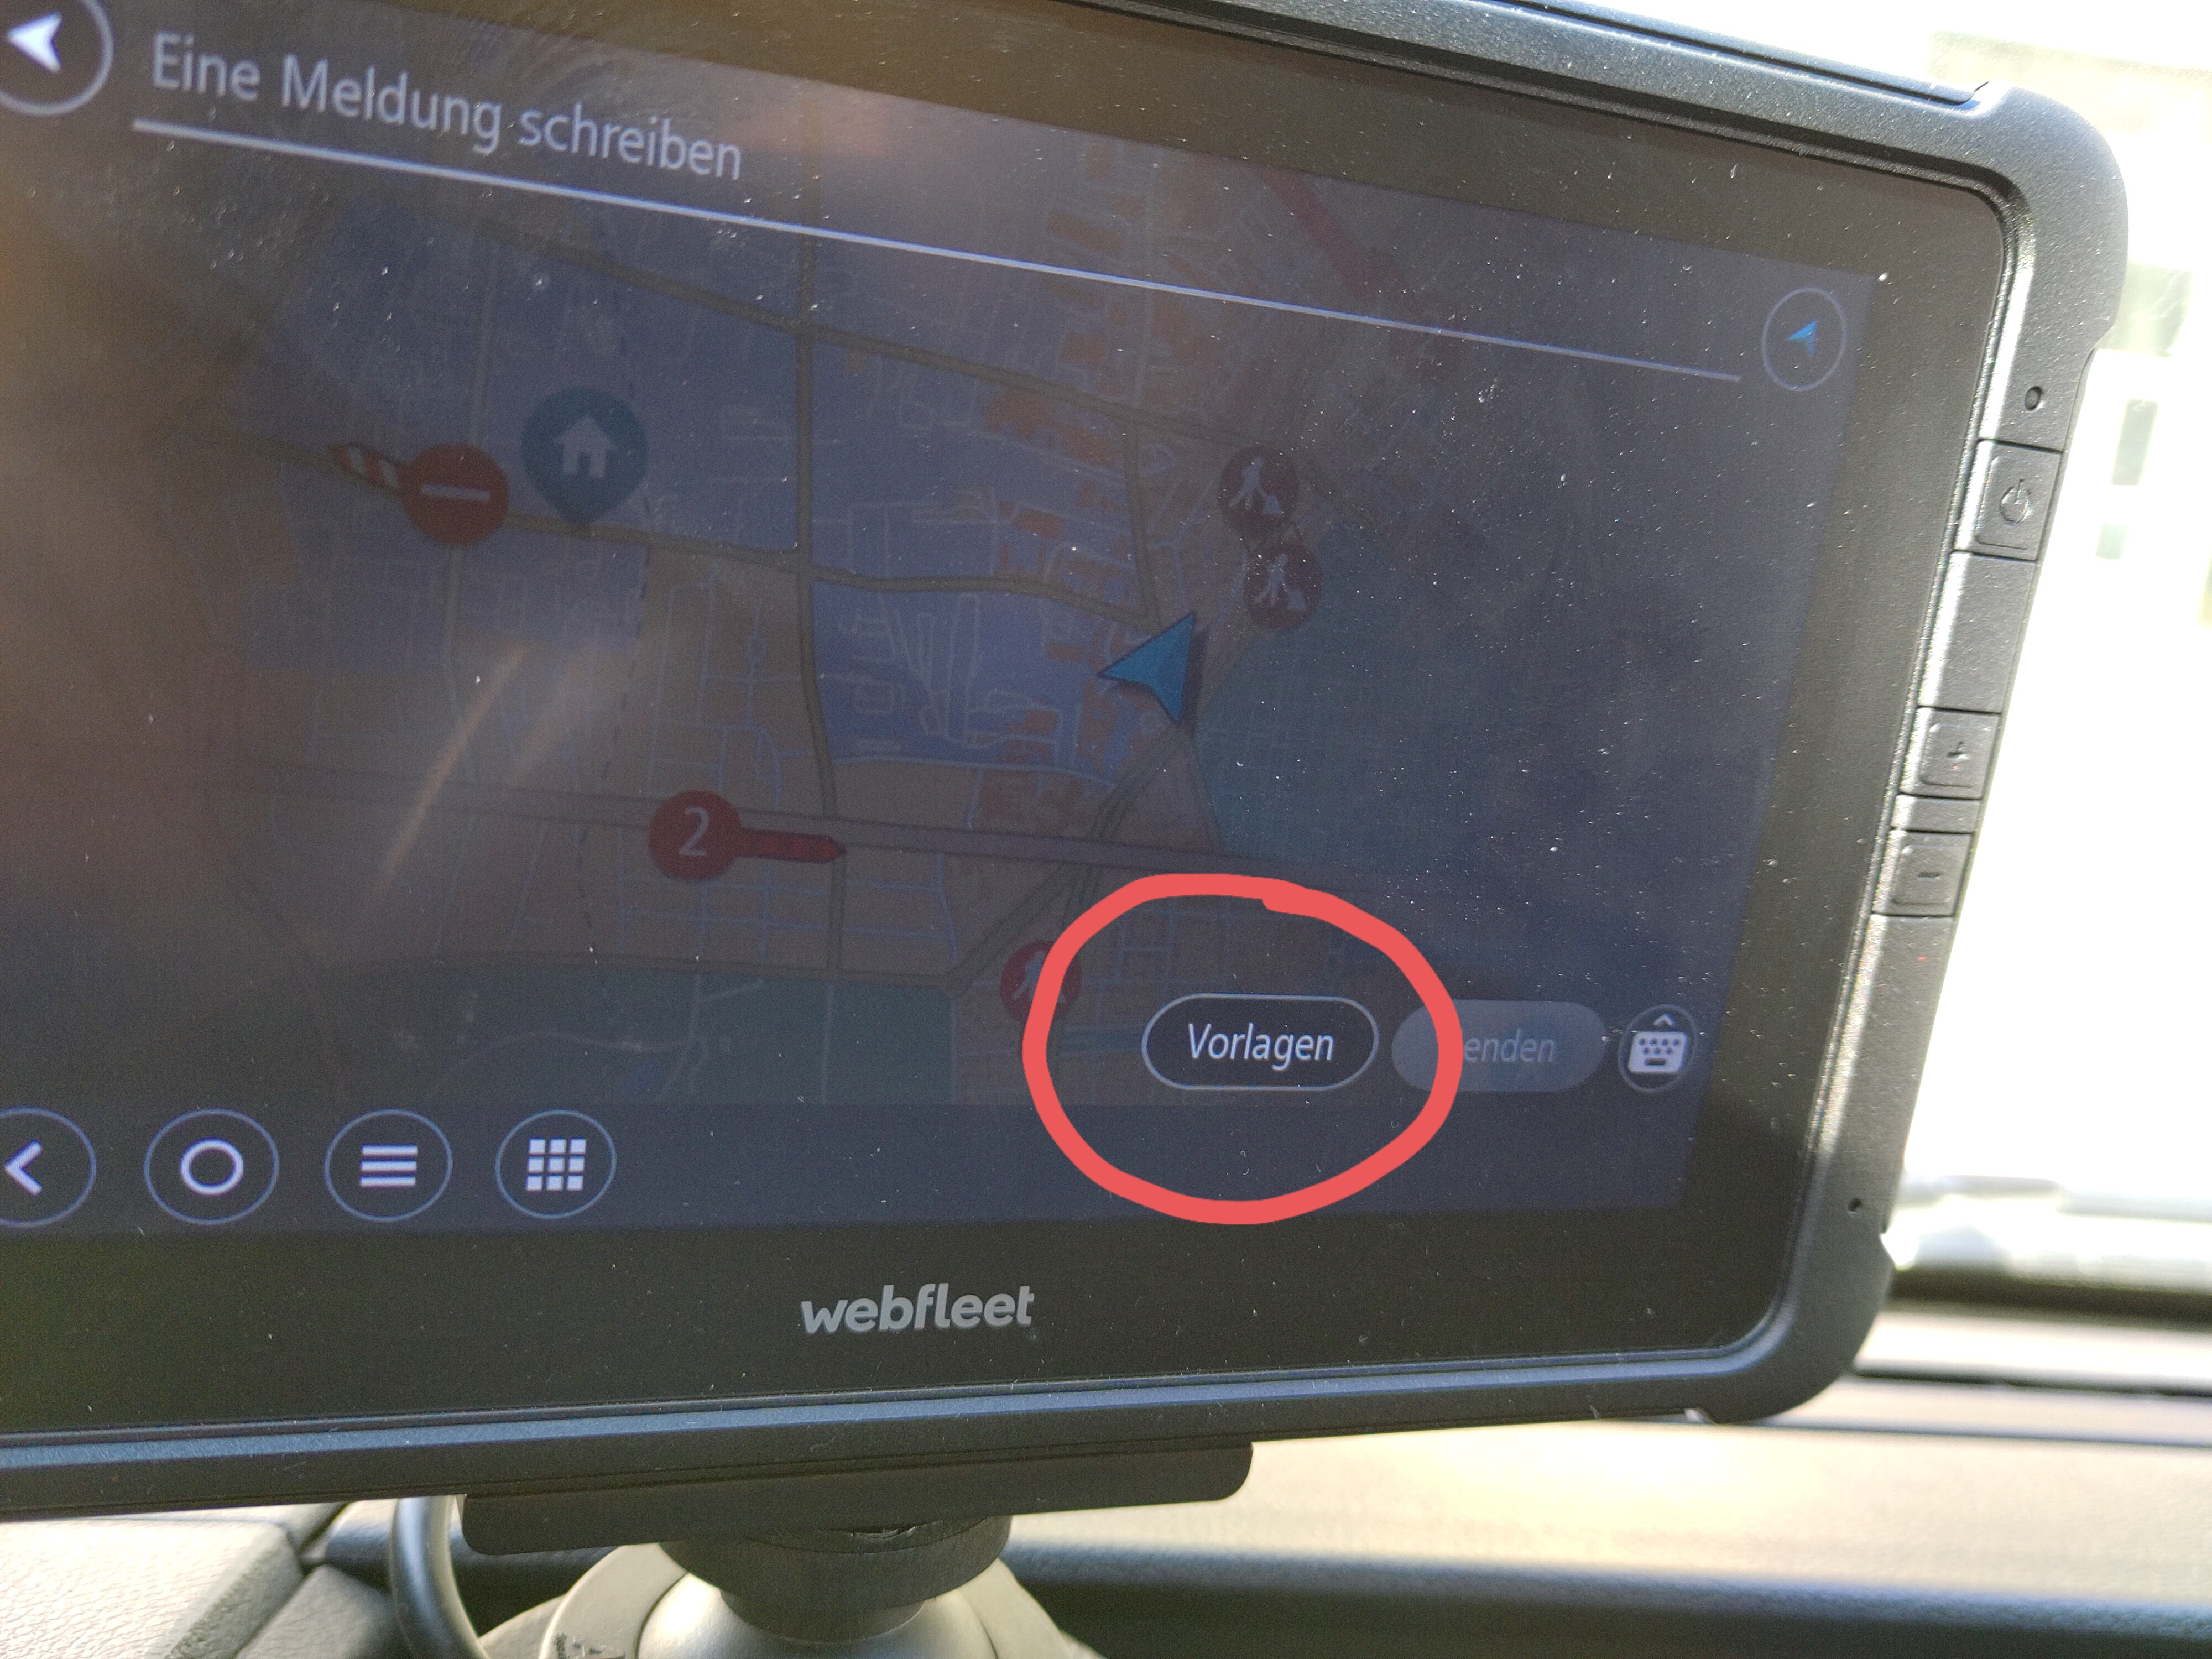
\includegraphics[width=5cm]{bilder/Schritt3.jpg}
            \caption{Schritt 3 Vorlagen}
            \label{Vorlagen}
        \end{center} 
    \end{figure}

    \subsection{Schrit 4 Statigabe}
    Im letzten Menü wählt ihr den gewünschten Stauts aus, z.B. Sprechwunsch wenn ihr etwas mit der Leitstelle
    klären möchtet. Oder korriegiert euren zuvor flasch gegeben Status auf den gewünschten.
    \begin{figure}[h]
        \begin{center}
            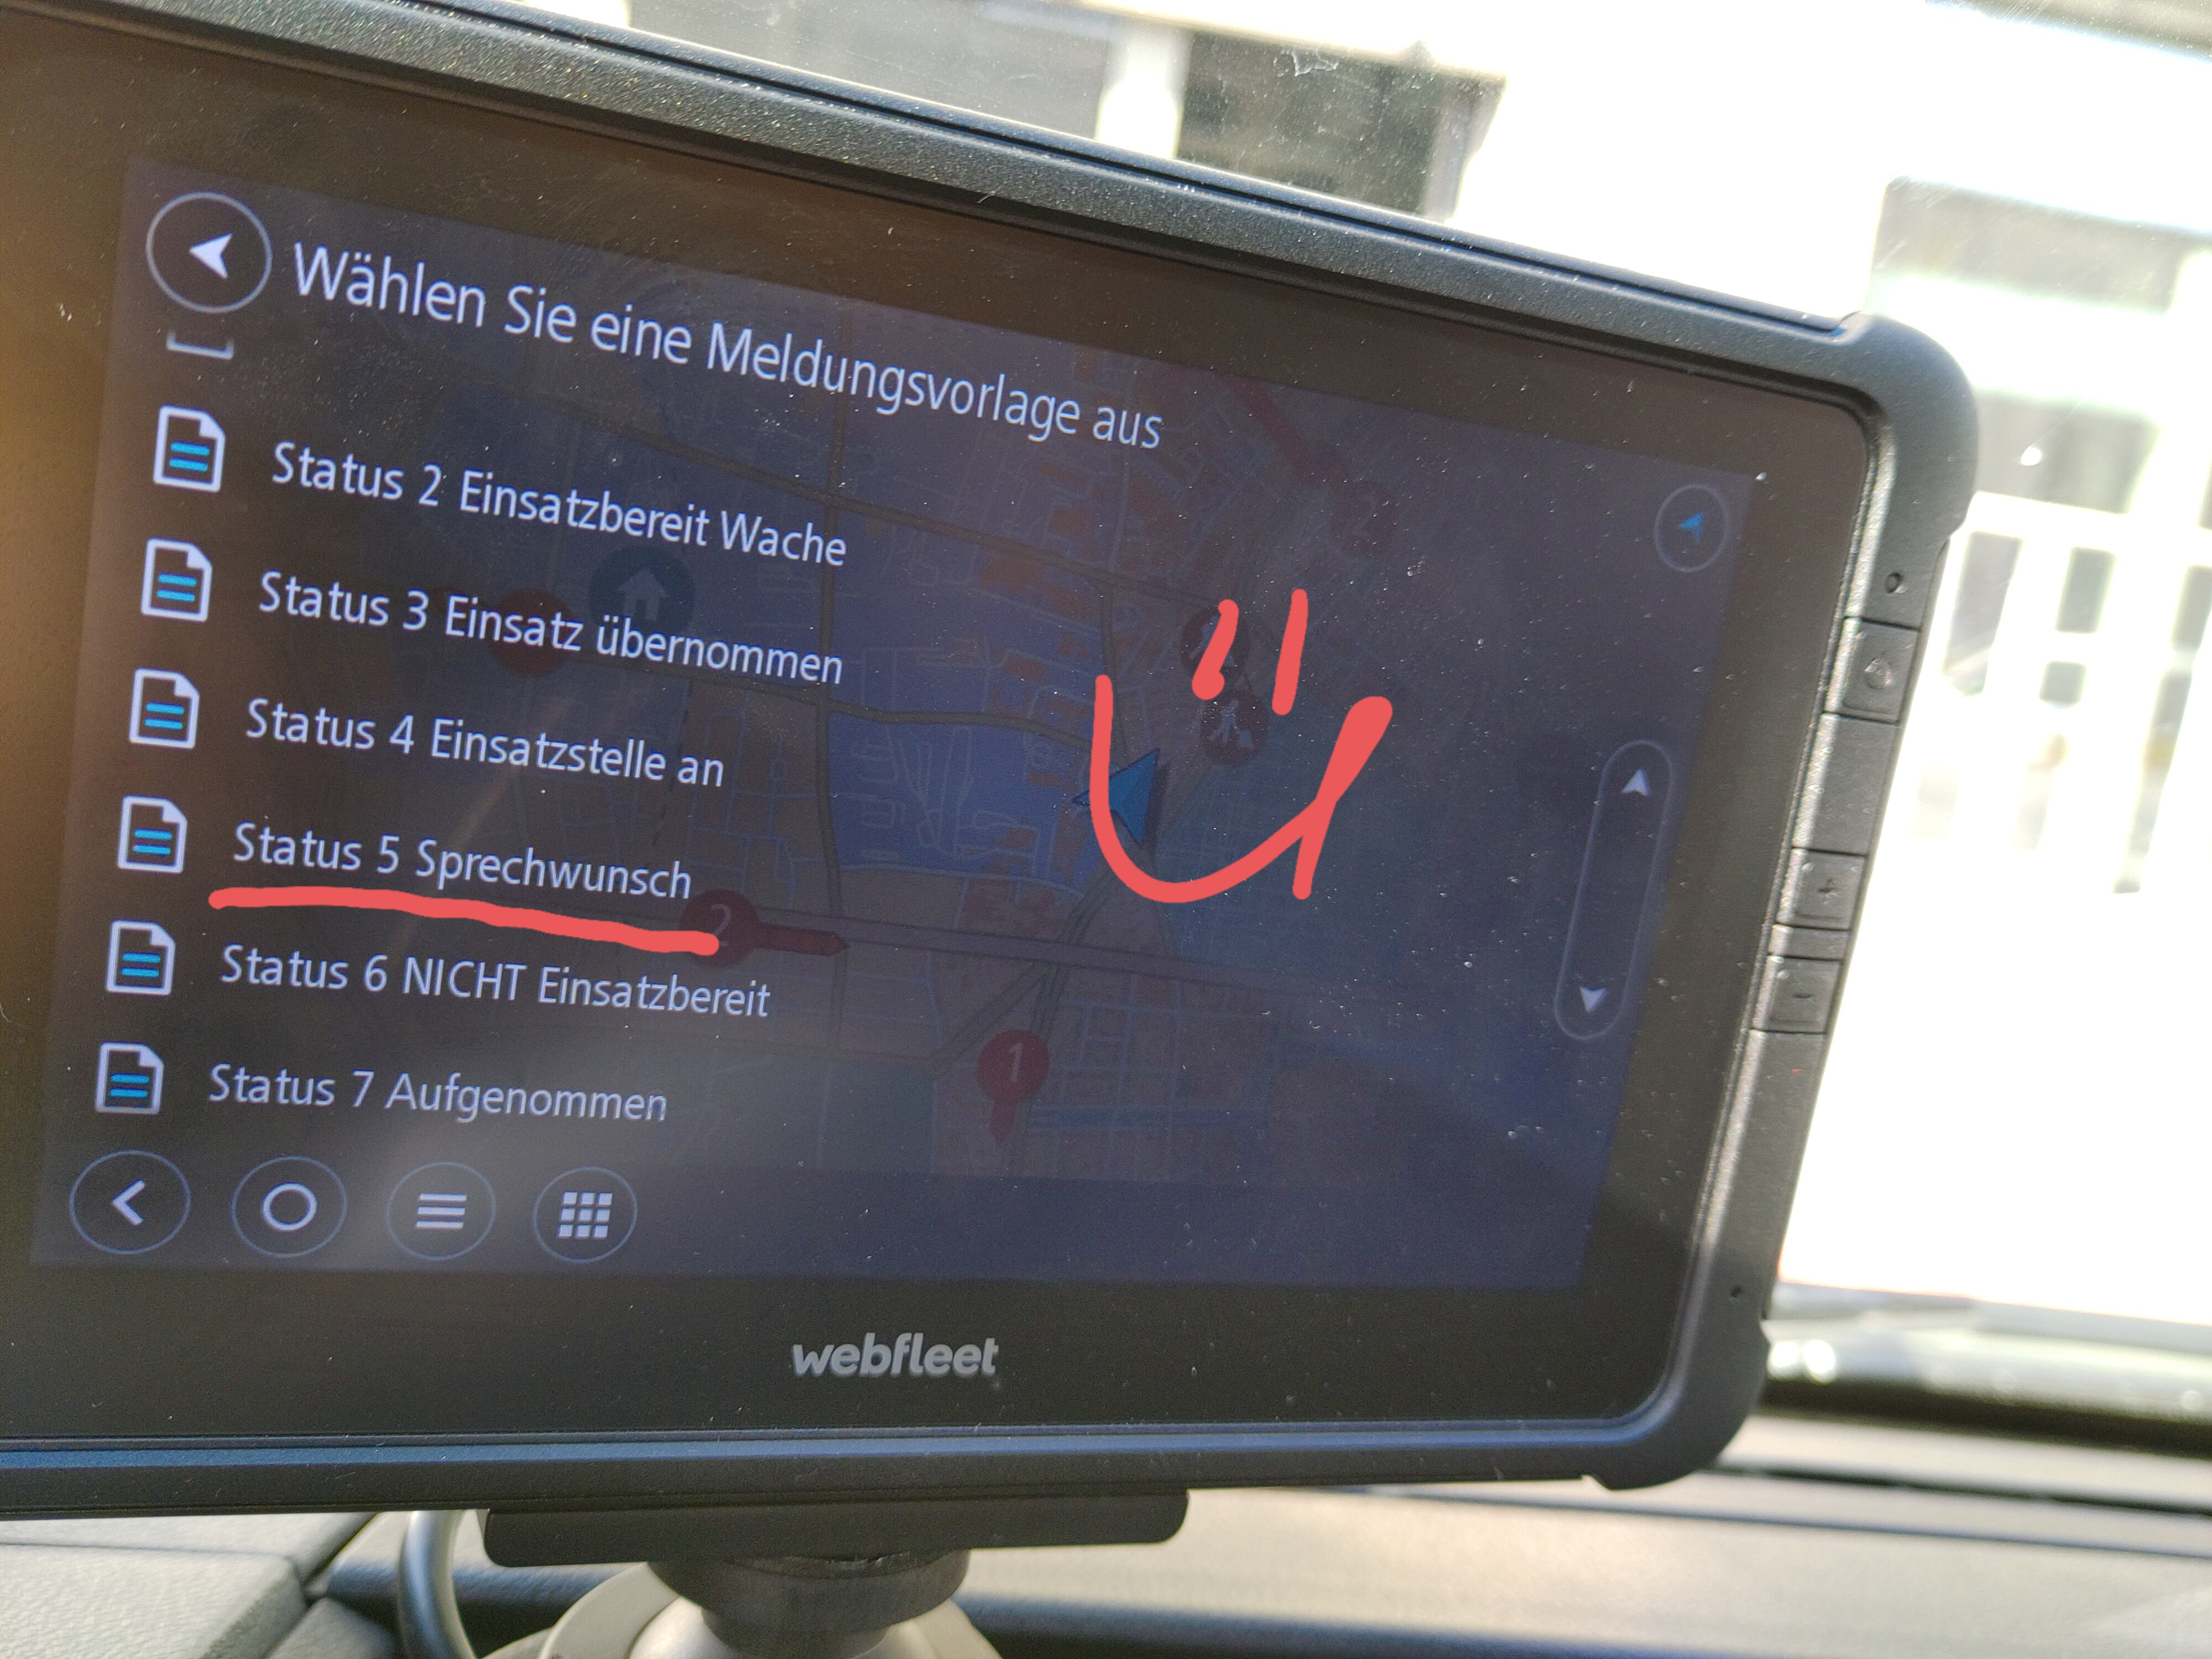
\includegraphics[width=5cm]{bilder/Schritt4.jpg}
            \caption{Schritt 4 Statigabe}
            \label{Statigabe}
        \end{center} 
    \end{figure}




\end{document}